\section{word2vec Embedding}\nocite{vulndetection}
\subsection{\textbf{Creating the Corpus}}

The first step is to create the corpus after cloning the repository from GitHub. We must install the required library for this class, which is \href{https://pydriller.readthedocs.io/en/latest/}{PyDriller}. 
\newline
PyDriller is a Python framework that helps developers on mining software repositories. With PyDriller, you can easily extract information from any Git repository, such as commits, developers, modifications, diffs, and source codes, and quickly export CSV files. \cite{pydriller}
\newline
PyDriller helps this class extract all commits from the GitHub repositories, which is the essential part of this repository. As mentioned in the exercise sheet, we have extracted all commits with the PyDriller from the following repositories.
\begin{itemize}
    \item \href{https://github.com/numpy/numpy}{NumPy}
    \item \href{https://github.com/django/django}{Django}
    \item \href{https://github.com/scikit-learn/scikit-learn}{sci-kit-learn}
    \item \href{https://github.com/tensorflow/tensorflow}{TensorFlow}
    \item \href{https://github.com/scipy/scipy}{scipy}
    \item \href{https://github.com/pallets/flask}{flask}
    \item \href{https://github.com/sqlmapproject/sqlmap}{sqlmap}
    \item \href{https://github.com/docker/compose}{compose}
\end{itemize}
We must remember that there are some changes in the PyDriller library since it was used for this repository. The changes are as follows:
\begin{enumerate}
    \item The \textit{RepositoyrMinning} class changed to \textit{Repository} \newline \textbf{Repository} is the main class of Pydriller, responsible for returning the list of commits you want. One of the main advantages of using PyDriller to mine software repositories is that it is highly configurable. We will now see all the options one can pass to the Repository.

    \item The \textit{modifications} method of RepositoyrMinning changed to 
        \textit{modified\_files} object. \newline We can get a list of modified files as well as their diffs and current source code from each commit. All Modifications can be obtained by iterating over the ModifiedFile object.
\end{enumerate}

After extracting the data from GitHub repositories, it will be saved in a specific file, \textit{pythontraining.txt} in the w2v. The result is shown in Figure \ref{fig: Figure1}.

\begin{figure}[!ht]
    \centering
    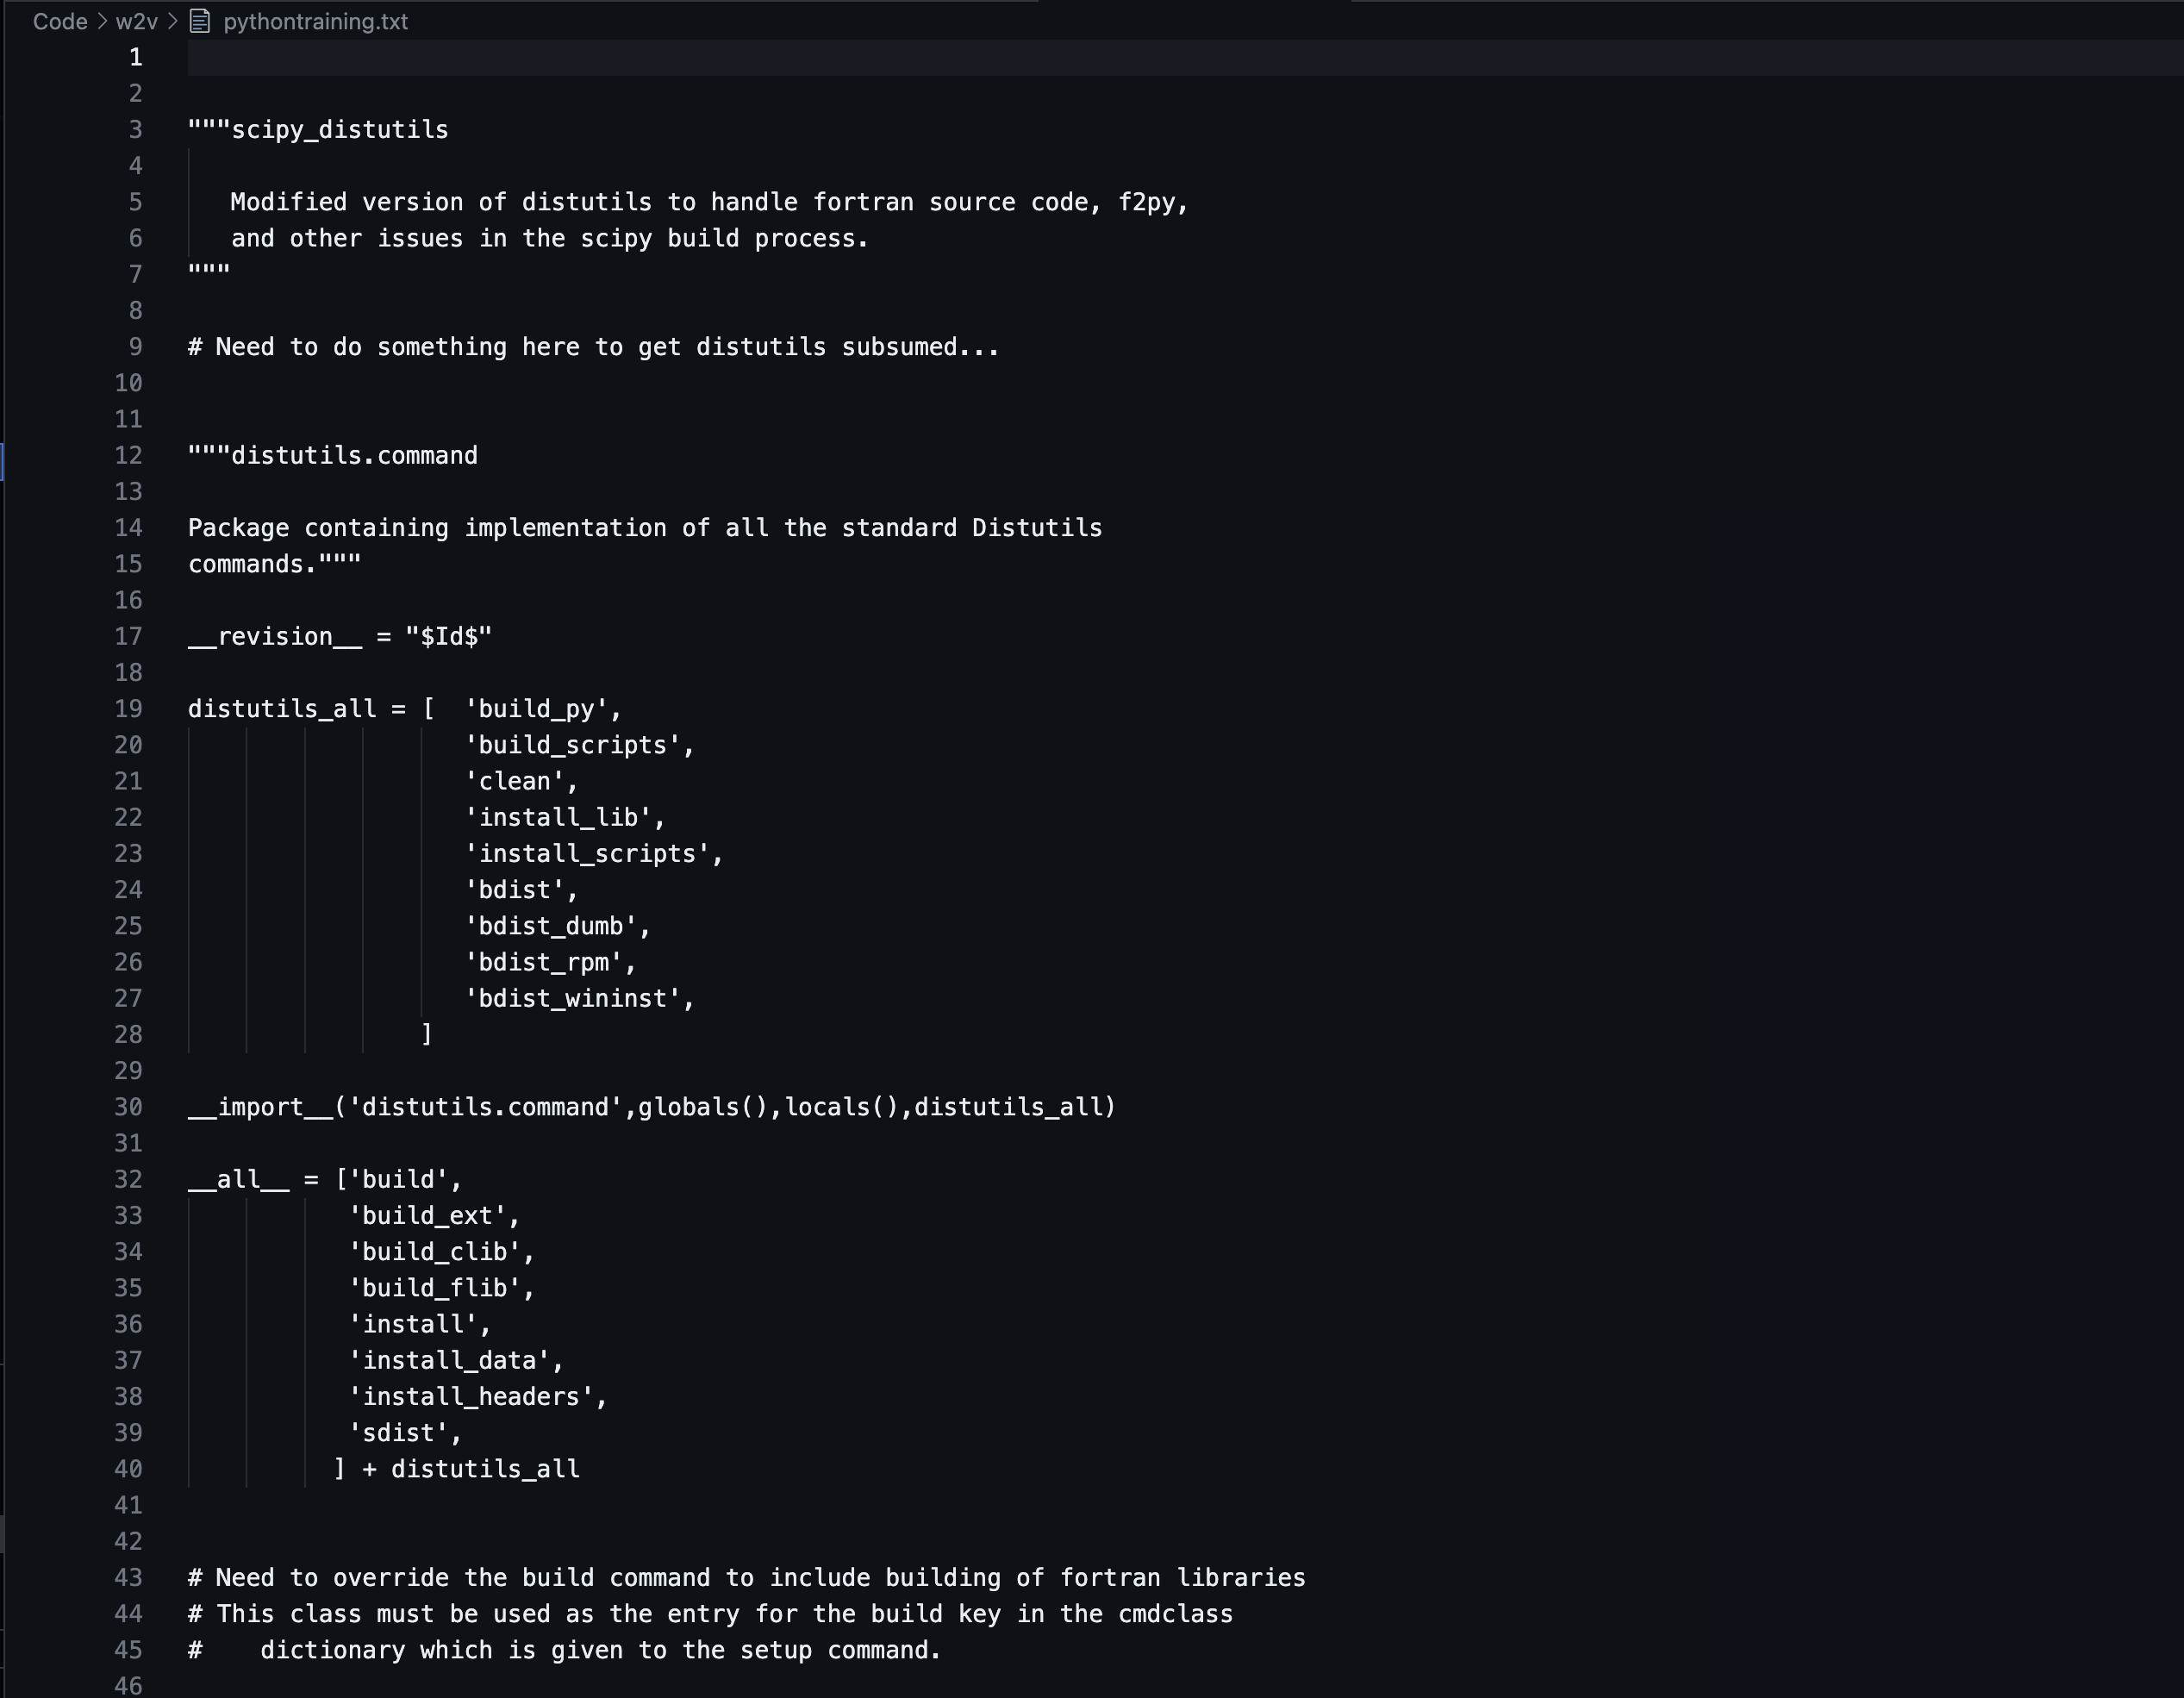
\includegraphics[width=1\linewidth]{pictures/py_training.png}
    \caption{Mined Data From GitHub Repositories}
    \label{fig: Figure1}
\end{figure}

\subsection{\textbf{Fixing Syntax Error}}
We have worked on the "w2v\_cleancorpus.py" file for this part of the task. 
In the mentioned file, we have encountered only one issue: Importing the StringIO library. It is changed from the "StringIO" main library to an "io" library module.\ref{fig: Figure2} 
\begin{figure}[!ht]
    \centering
    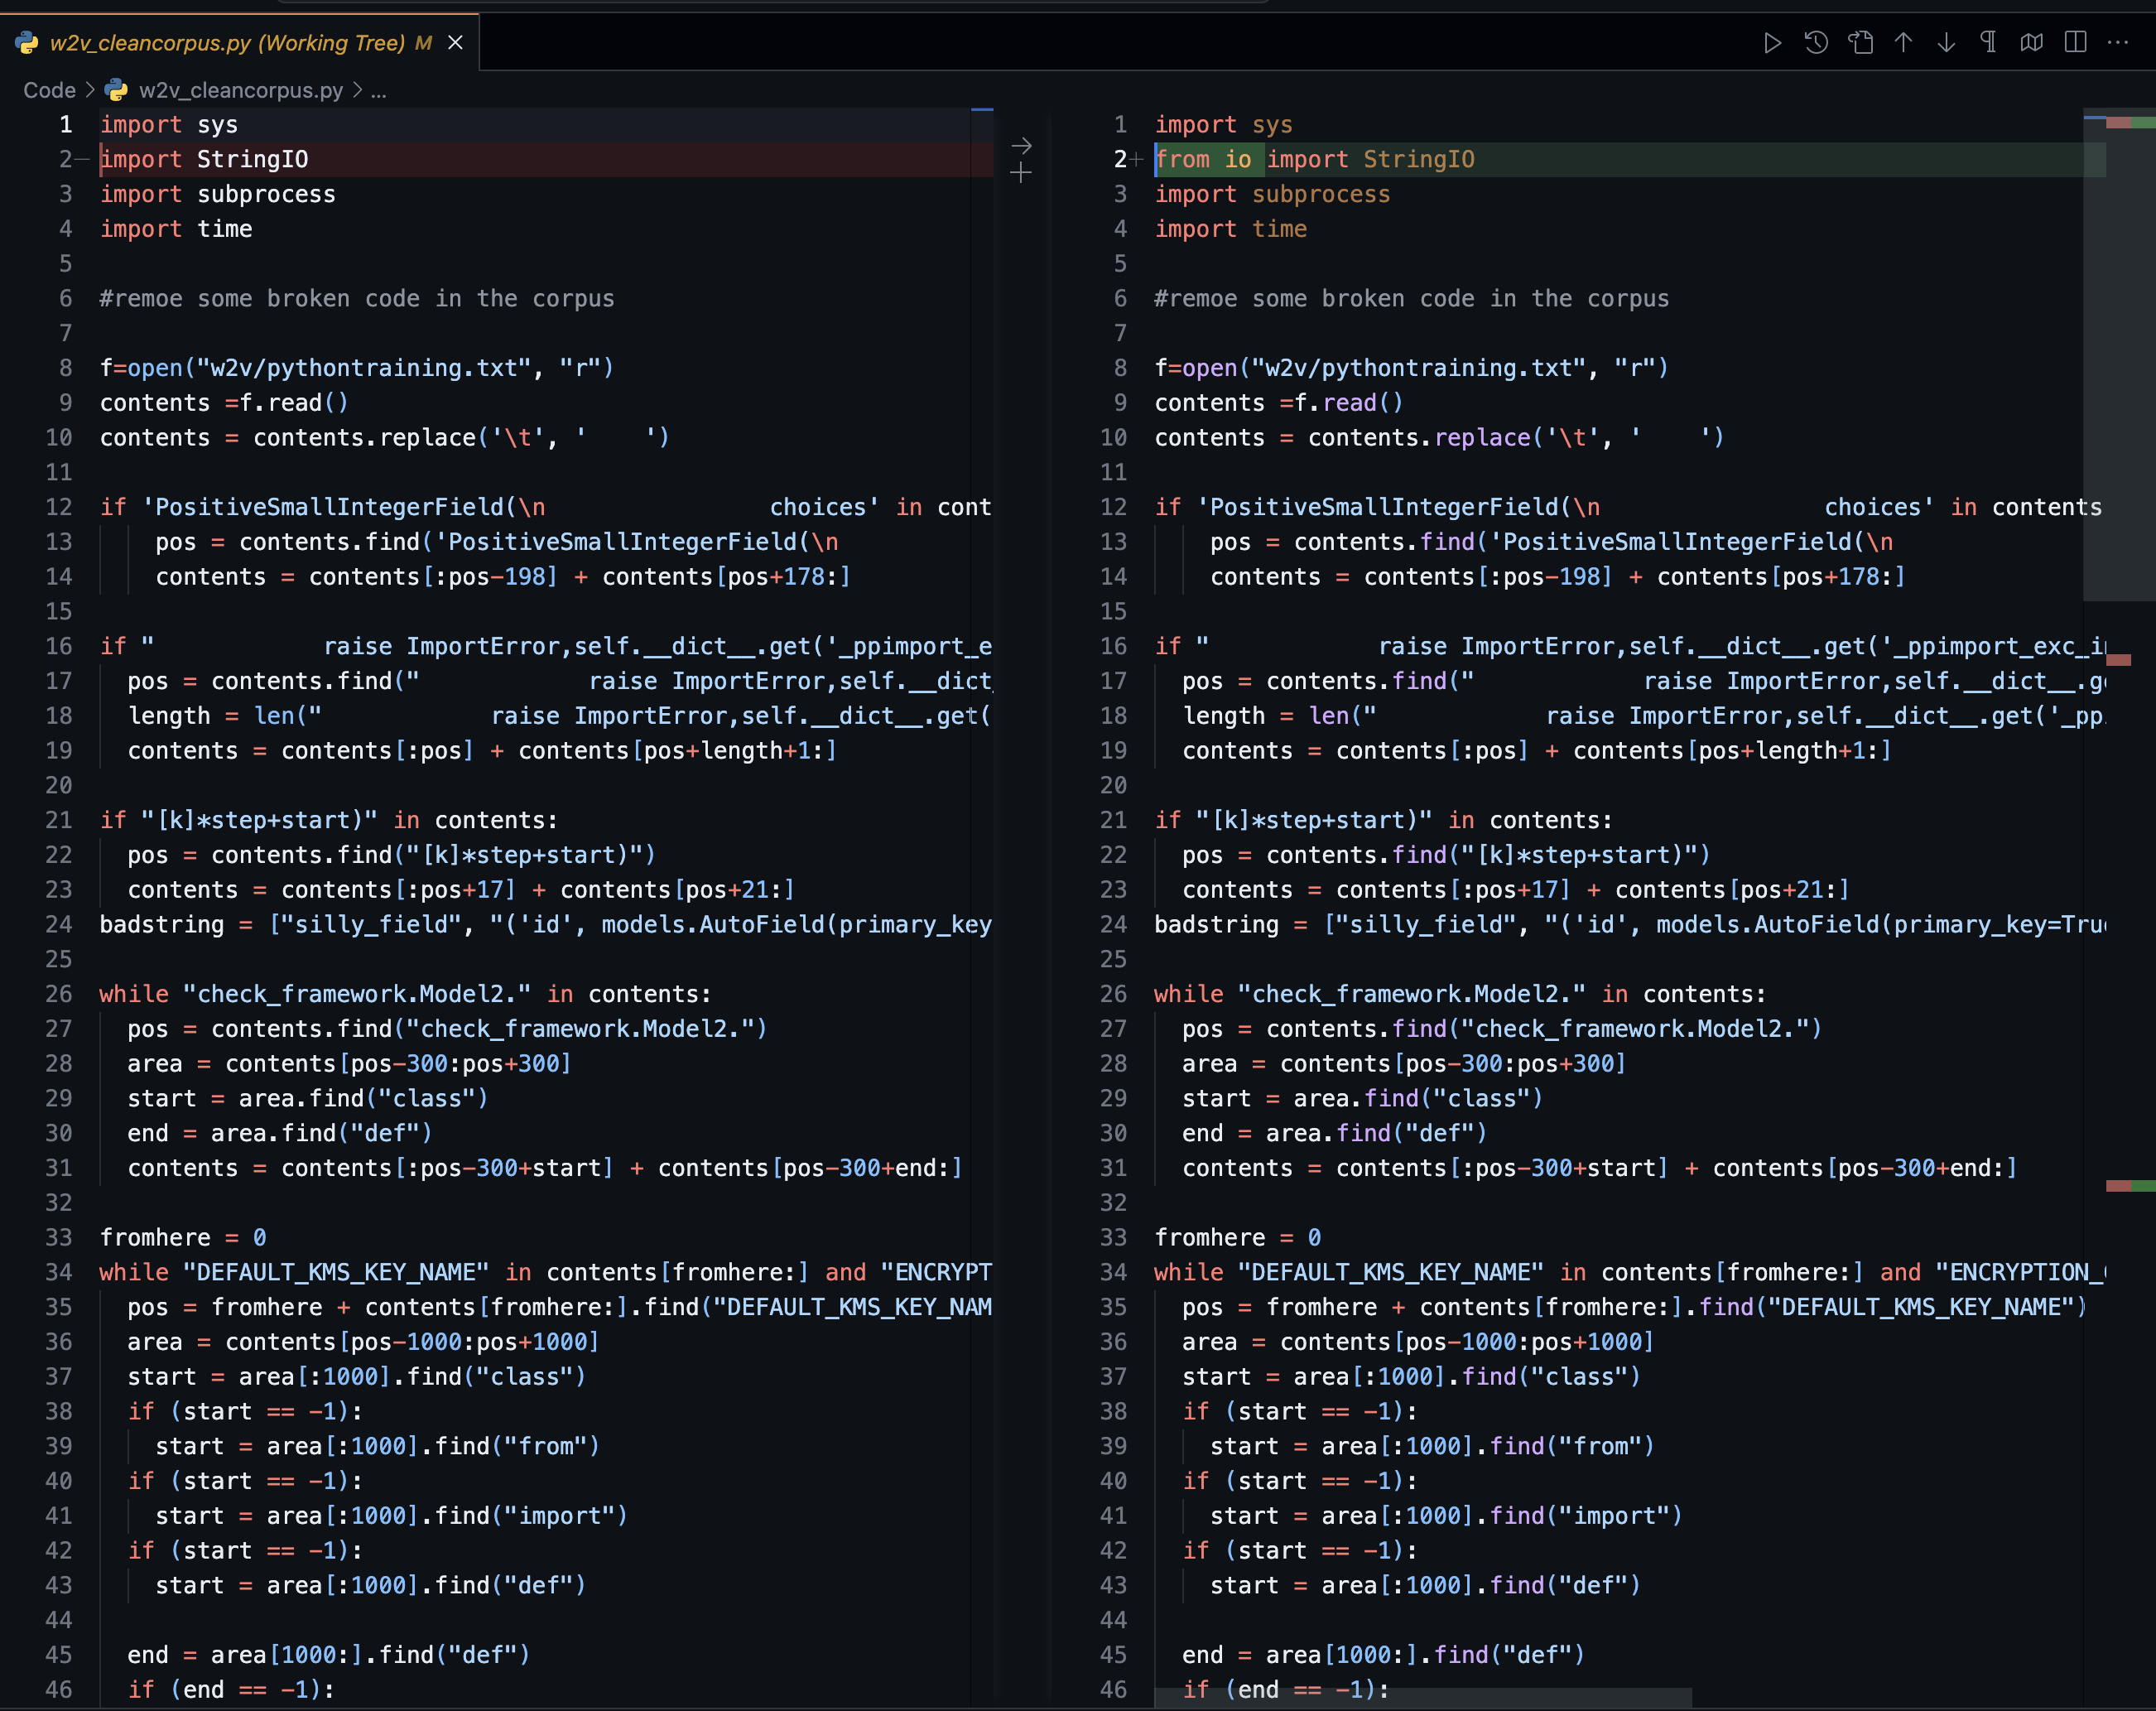
\includegraphics[width=1\linewidth]{pictures/cleancorpus_error.png}
    \caption{Cleancorpus file Issue}
    \label{fig: Figure2}
\end{figure}

After cleaning the mined data, the results are saved in the "pythontraining\_edit.txt". It is shown in Figure \ref{fig: Figure3}
\begin{figure}[!ht]
    \centering
    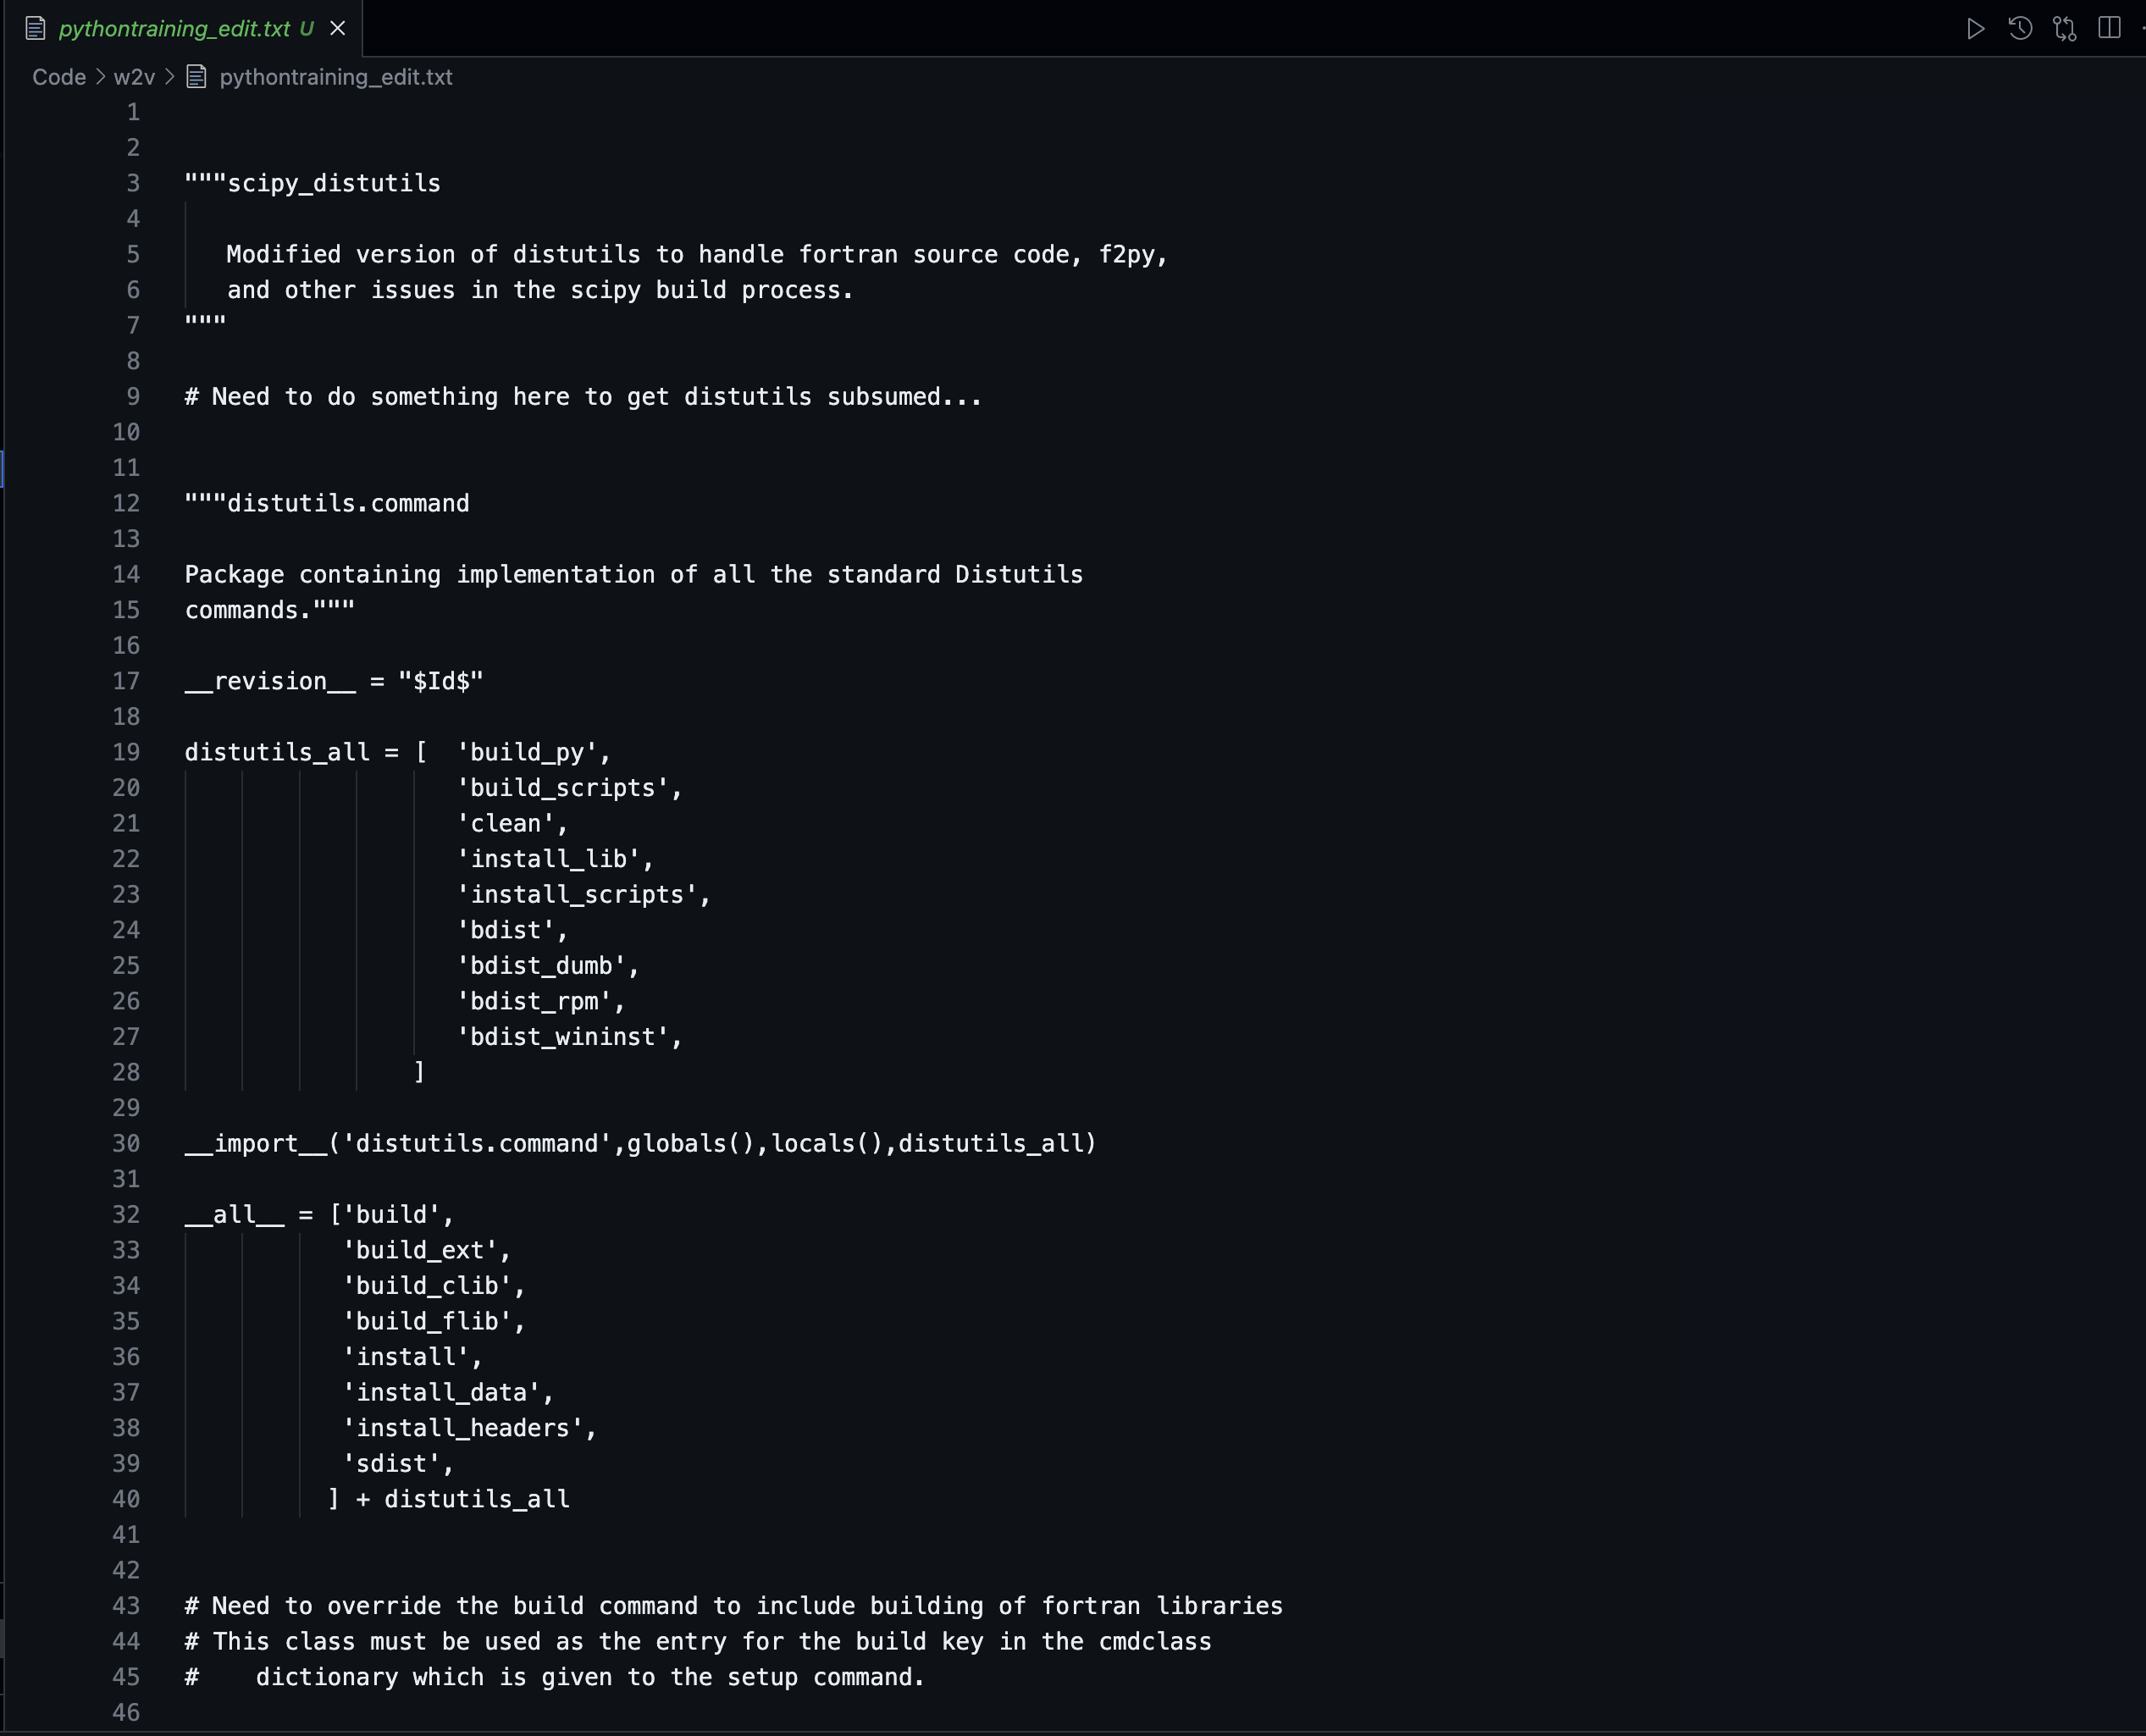
\includegraphics[width=1\linewidth]{pictures/cleaned_data.png}
    \caption{Cleaned Mined Data}
    \label{fig: Figure3}
\end{figure}

\subsection{\textbf{Tokenization}}
Tokenization is one of the essential steps; while using it, we have faced two issues. They are shown in Figure \ref{fig: Figure4}. 
\begin{enumerate}
    \item \textbf{"StringIO" to "io" as a submodule. }\newline When working with text data in Python, especially when dealing with files or streams, the "io" module provides a range of classes and functions to handle input and output operations. "StringIO" is a class in the "io" module that allows you to treat strings as file-like objects. However, if you need to convert the contents of a "StringIO" object to a regular string, you can use the \textit{.getvalue()} method.
    \item \textbf{"\textit{StringIO.StringIO(out)}" method to "\textit{StringIO(out.decode('utf-8'))}"} \newline In Python 3, the StringIO class is located in the io module, and it works with Unicode strings by default. If you have data in bytes format (encoded in UTF-8, for example) and you want to work with it as a string, you need to decode it into a Unicode string. You can achieve this by using the decode() method with the appropriate encoding, in this case, 'utf-8'.
\end{enumerate}

\begin{figure}[!ht]
    \centering
    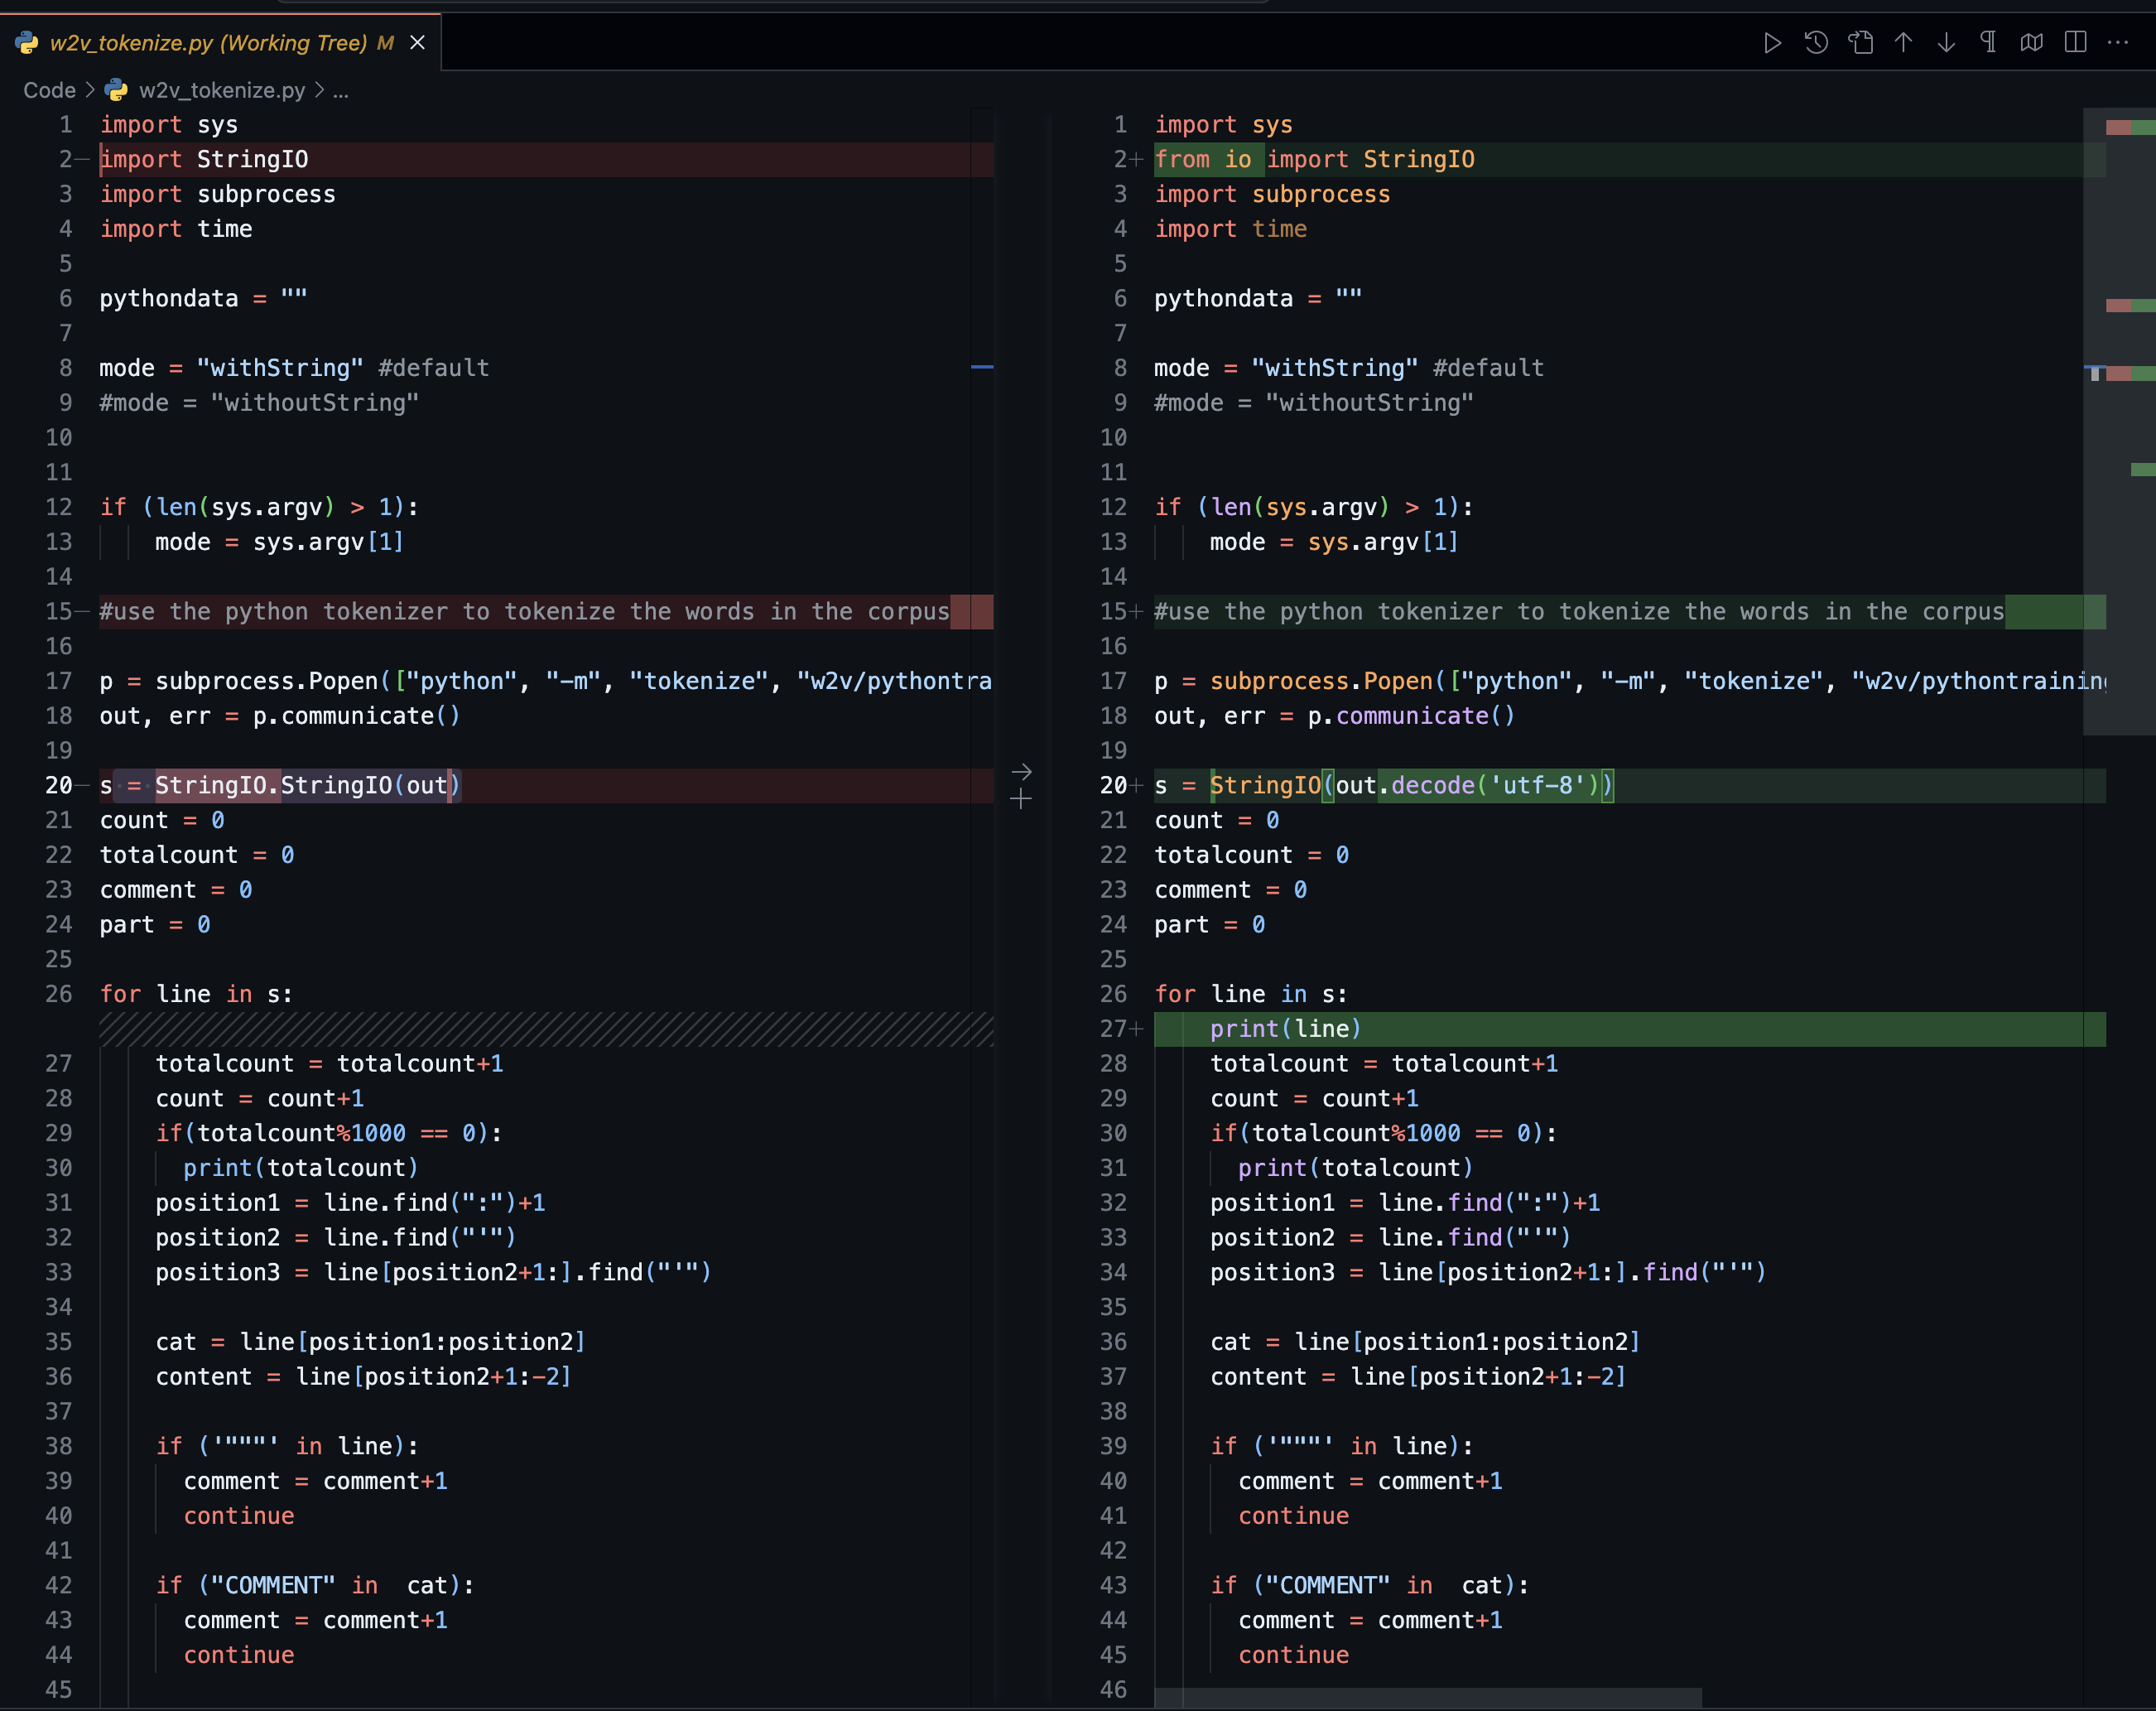
\includegraphics[width=1\linewidth]{pictures/tokenization_isseus.png}
    \caption{Tokenizer issues and solutions}
    \label{fig: Figure4}
\end{figure}

After solving them, we managed to generate the tokenized file. Because of its size, the tokenizer class is divided into 11 files. The saved files are shown in figure \ref{fig: Figure5}.
\begin{figure}[!ht]
    \centering
    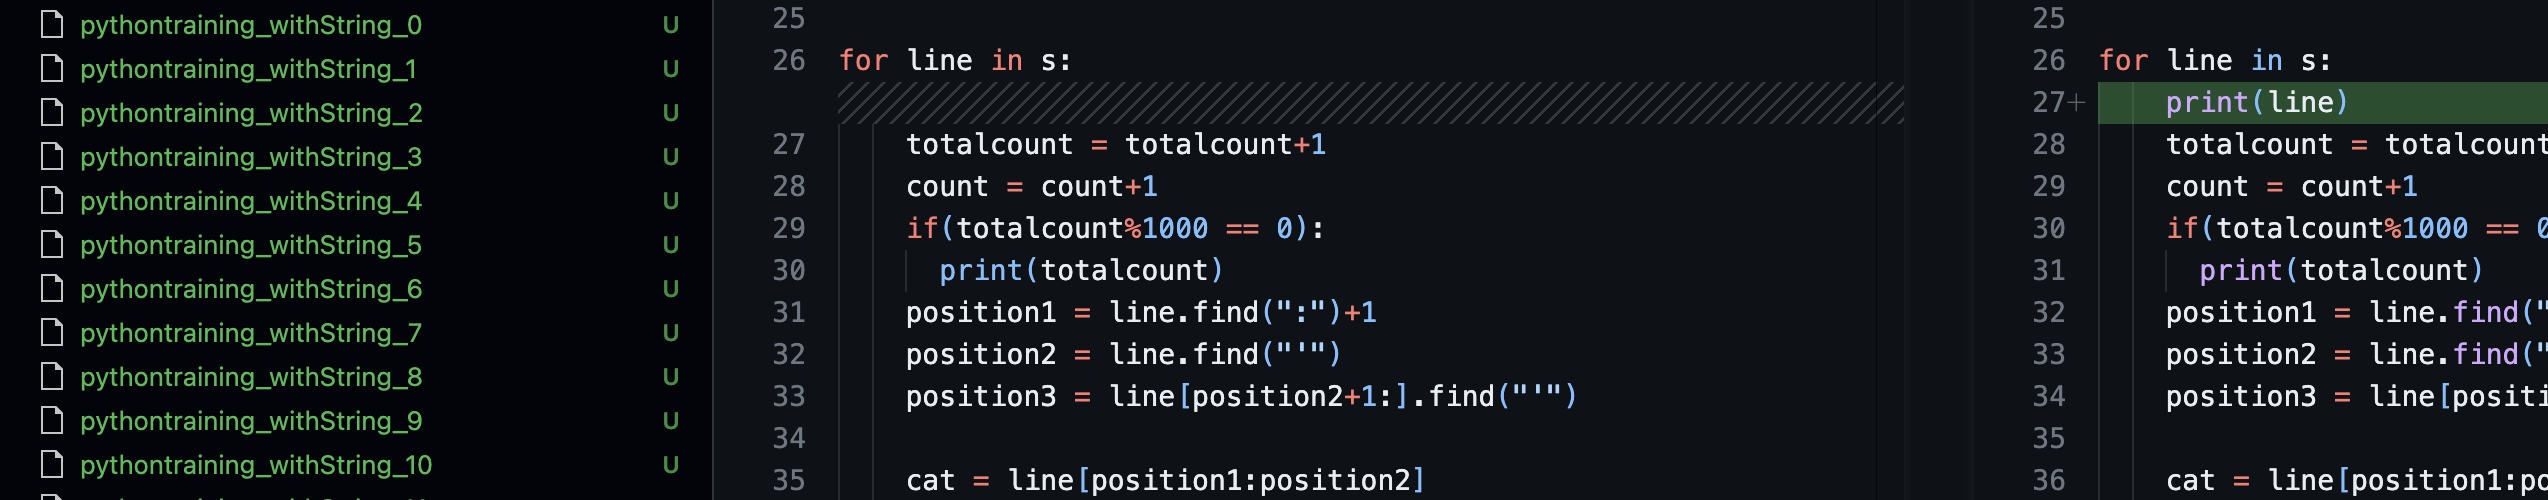
\includegraphics[width=1\linewidth]{pictures/tokenized_data.png}
    \caption{Tokenized data in separate files}
    \label{fig: Figure5}
\end{figure}

\begin{figure}
    \centering
    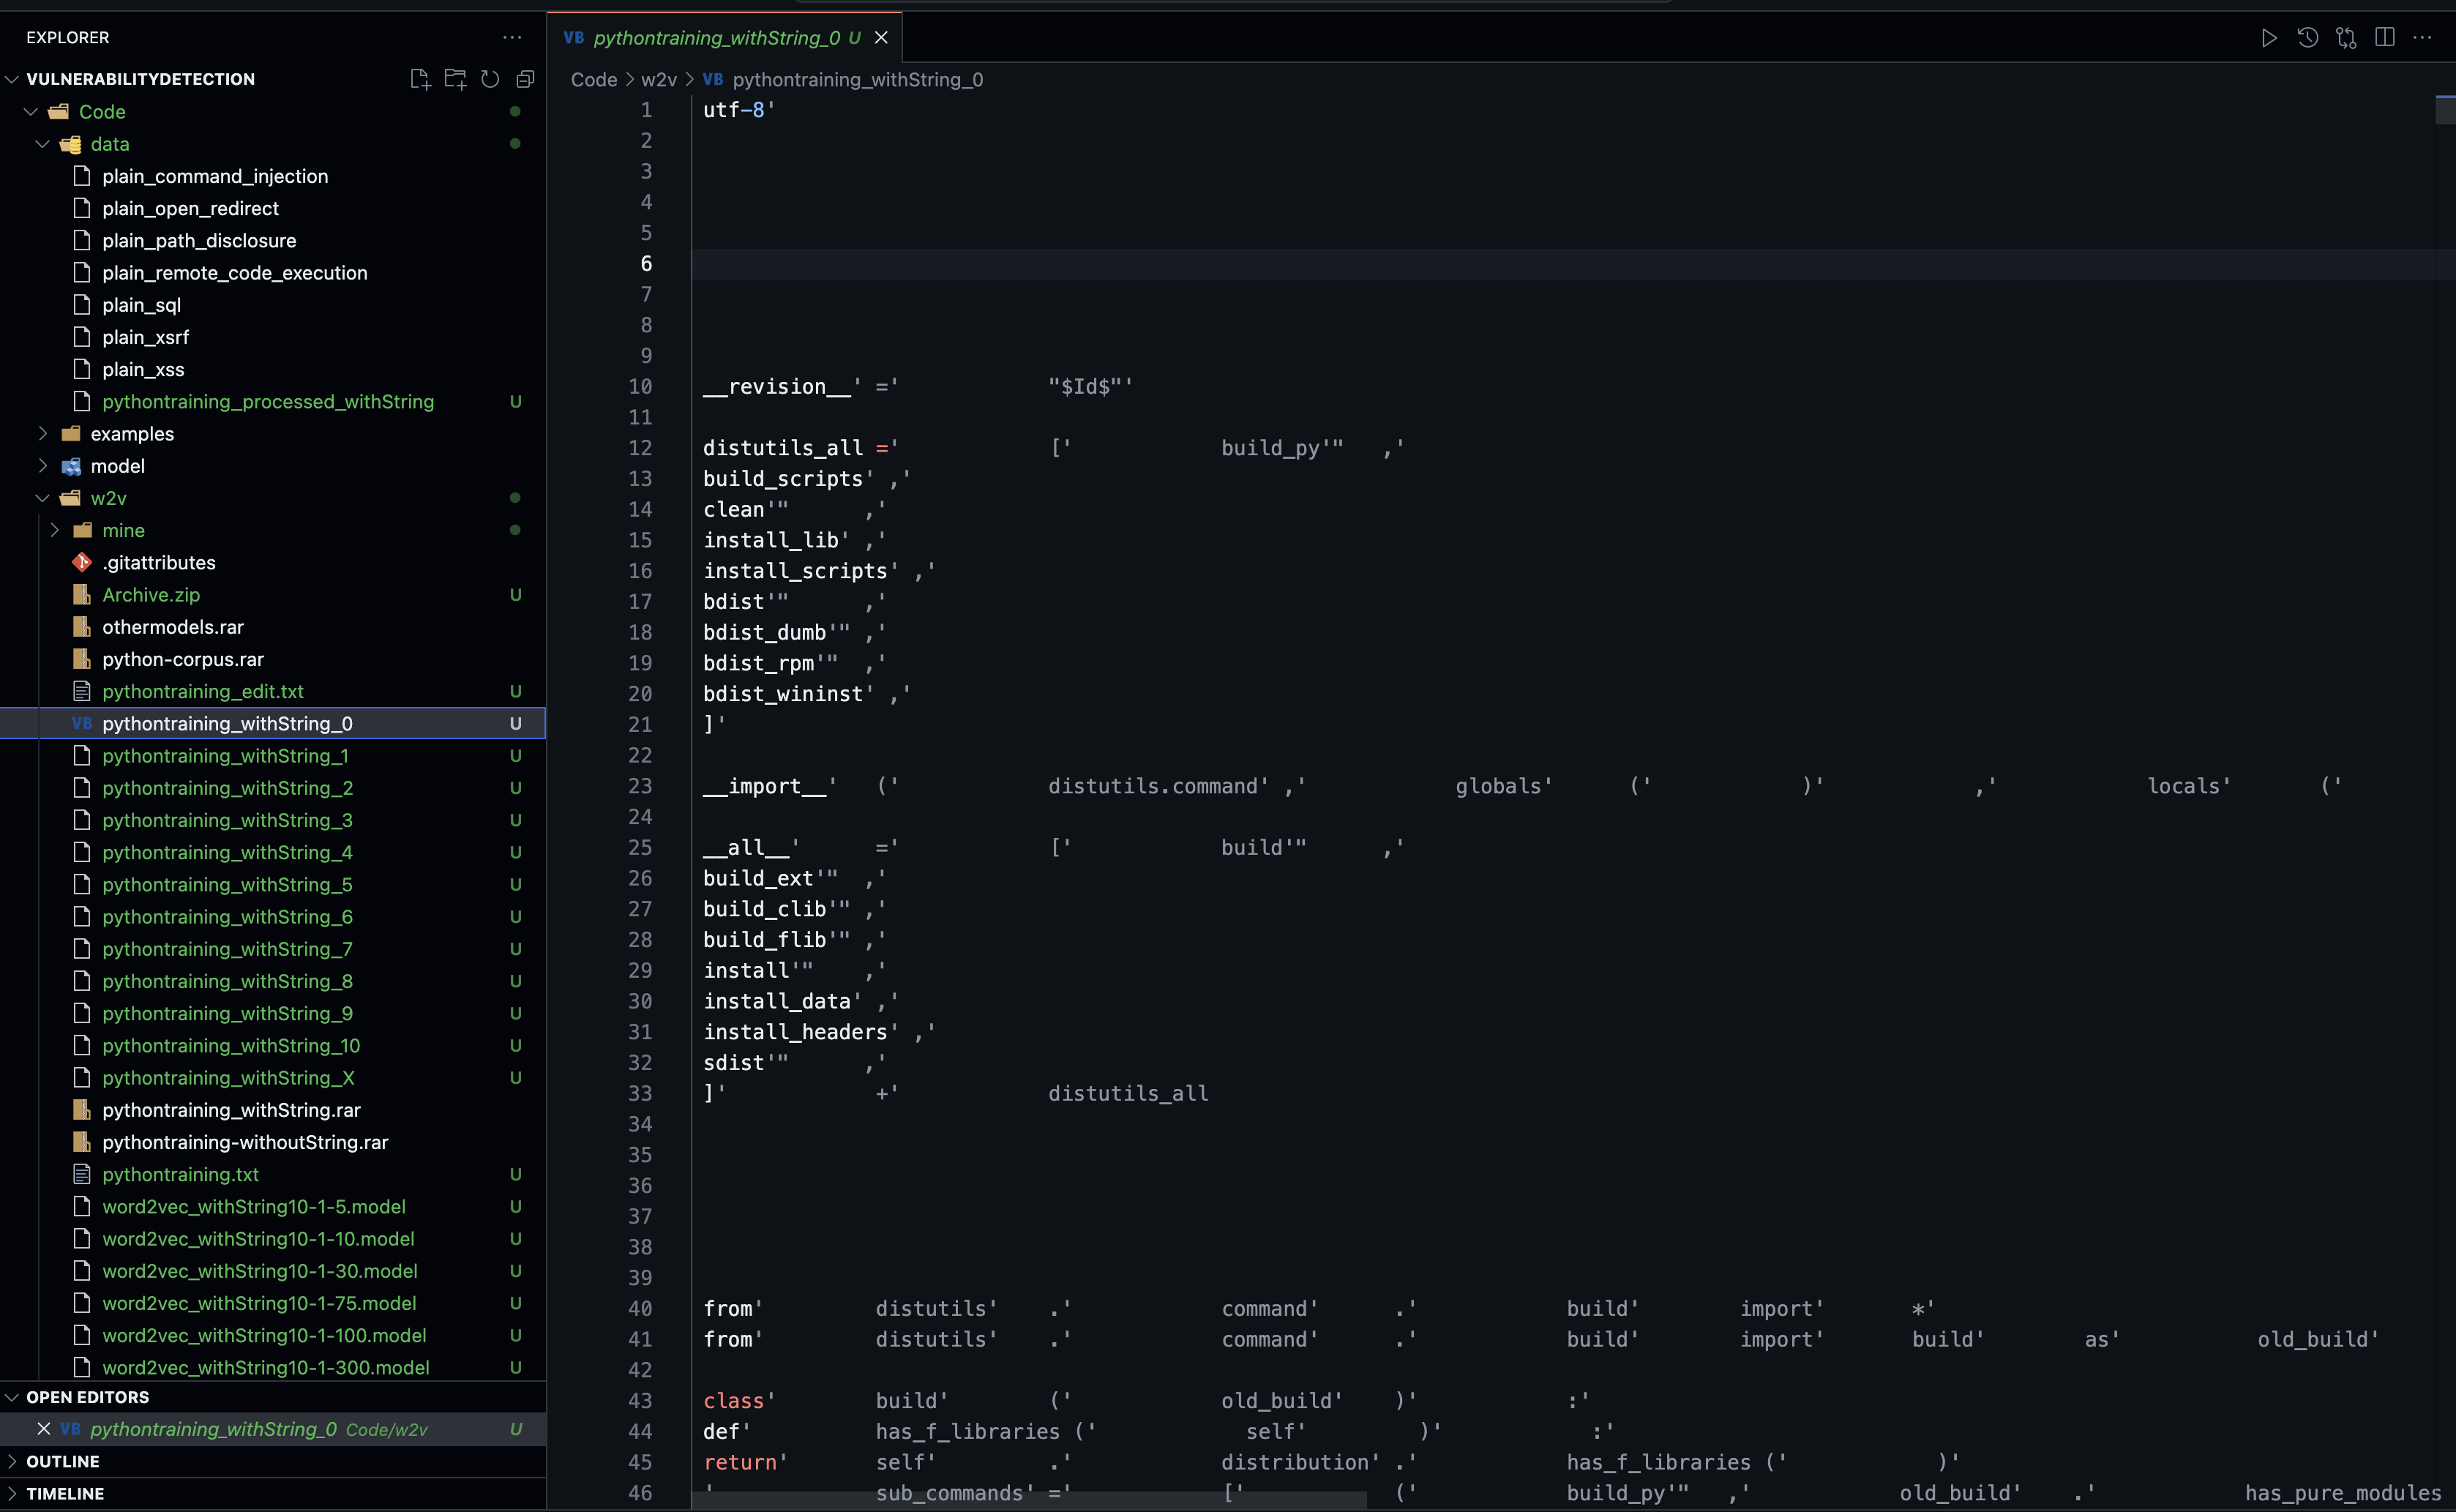
\includegraphics[width=1\linewidth]{pictures/tokenized_sample.png}
    \caption{Tokenized file sample}
    \label{fig: tokenize_sample}
\end{figure}

\subsection{\textbf{Merging Results}}
In this step, you can merge all tokenized data into one large file, which can be beneficial for training your model in the next step. To differentiate this large file from the individual tokenized files, "X" is appended to the end of its name.

While working with this file, we have faced with two issues:
\newline
\begin{enumerate}
 \item The "mode" data variable is missing. This variable saves the mode of tokenization, which has two values (WithString, WithoutString); we have used "WithString" as an exercise file description. We solved this issue by initializing the "mode" variable and assigning the value.
 \item The for loop value range from 0 to 71 was incorrect because we only needed a range of 0 to 10.  We have updated the code and added an exception. Whenever the program does not find the value, it will stop the loop and return the file with "X" at the end of it. Overall changes in this file are shown in Figure \ref{fig: Figure6}
\end{enumerate}

\begin{figure}
    \centering
    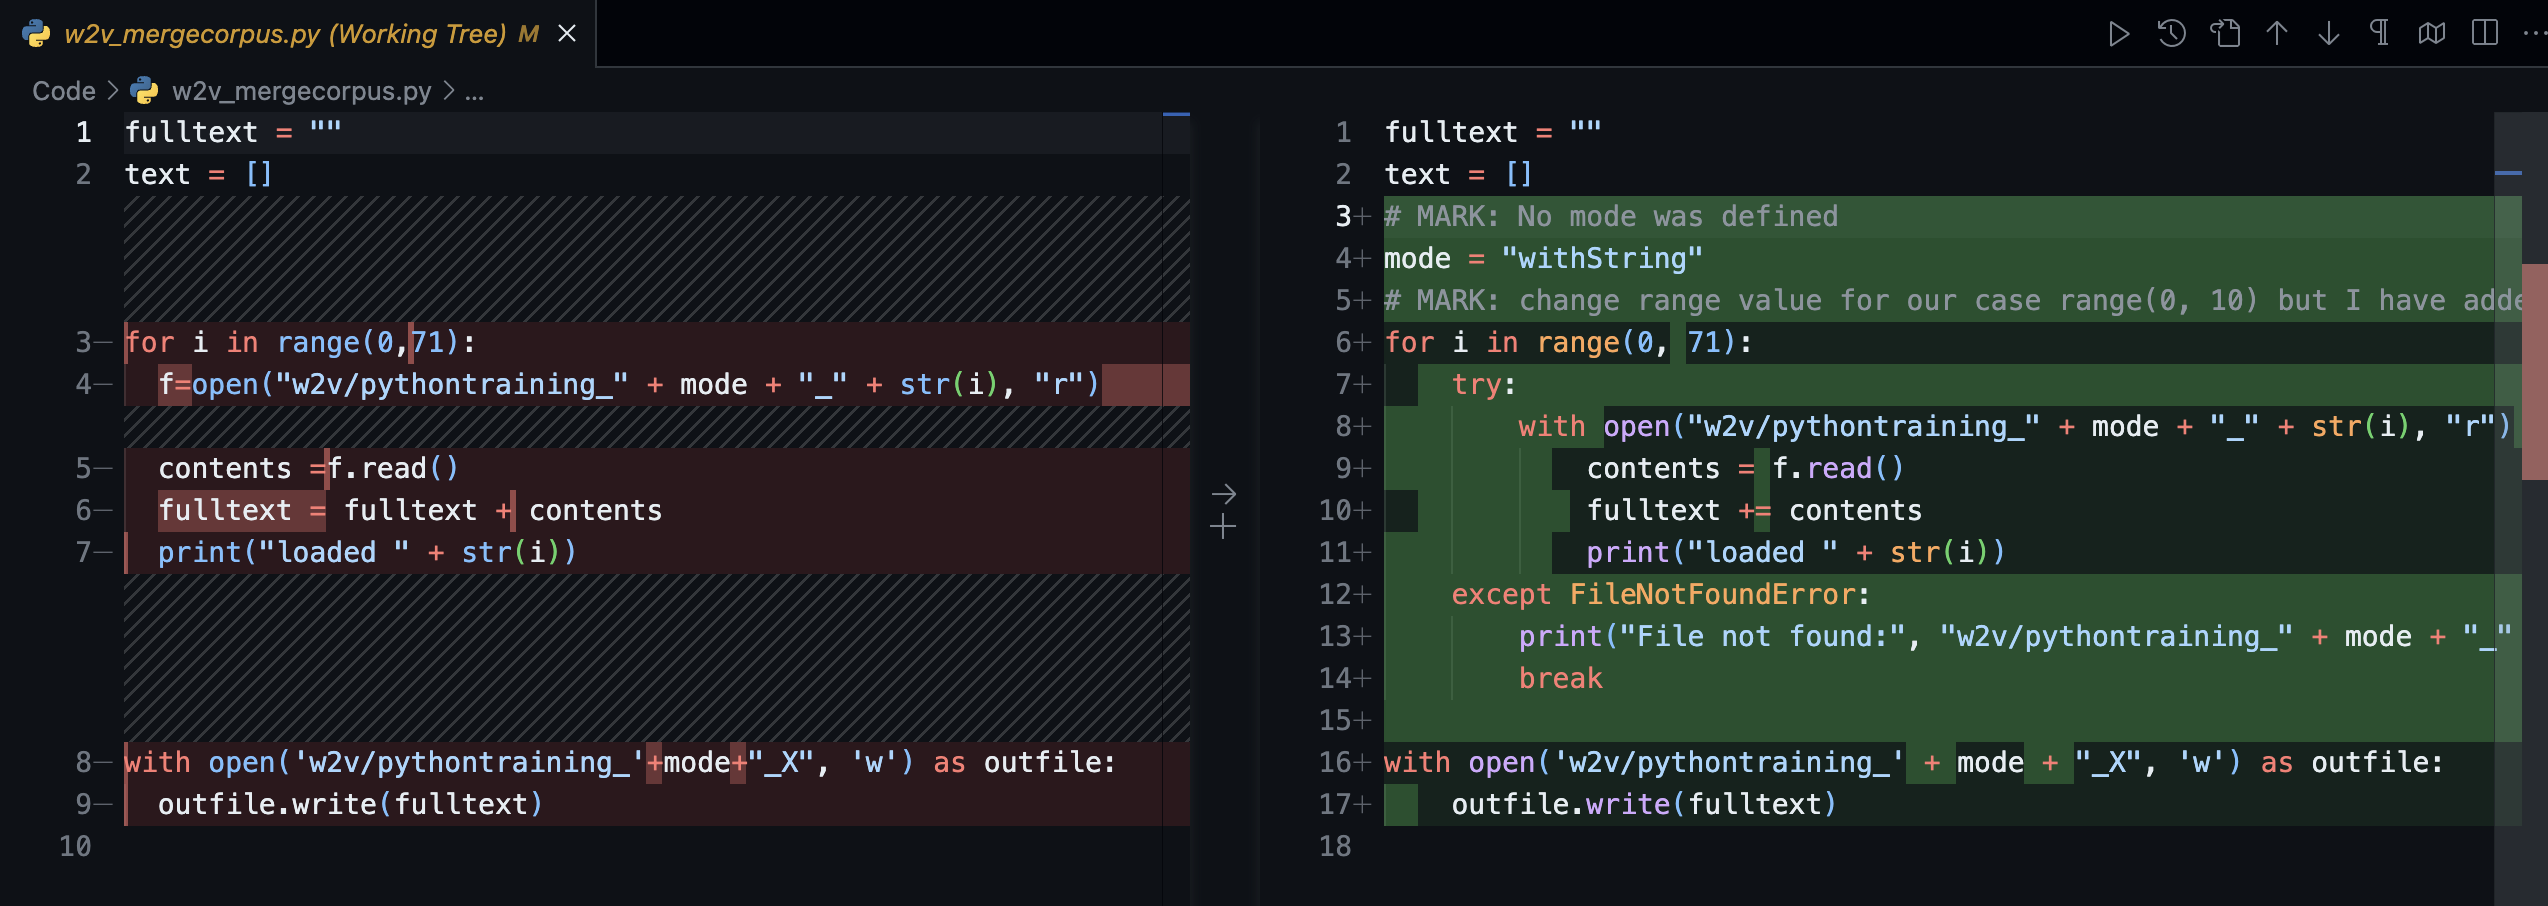
\includegraphics[width=1\linewidth]{pictures/mergin_issues.png}
    \caption{Merging file issues with solutions}
    \label{fig: Figure6}
\end{figure}

After successfully running the file, all 11 tokenized files merged into a large file and received the output. The output has been saved in the "pythontraining\_withString\_X" file, shown in \ref{fig: Figure7}.
\begin{figure}
    \centering
    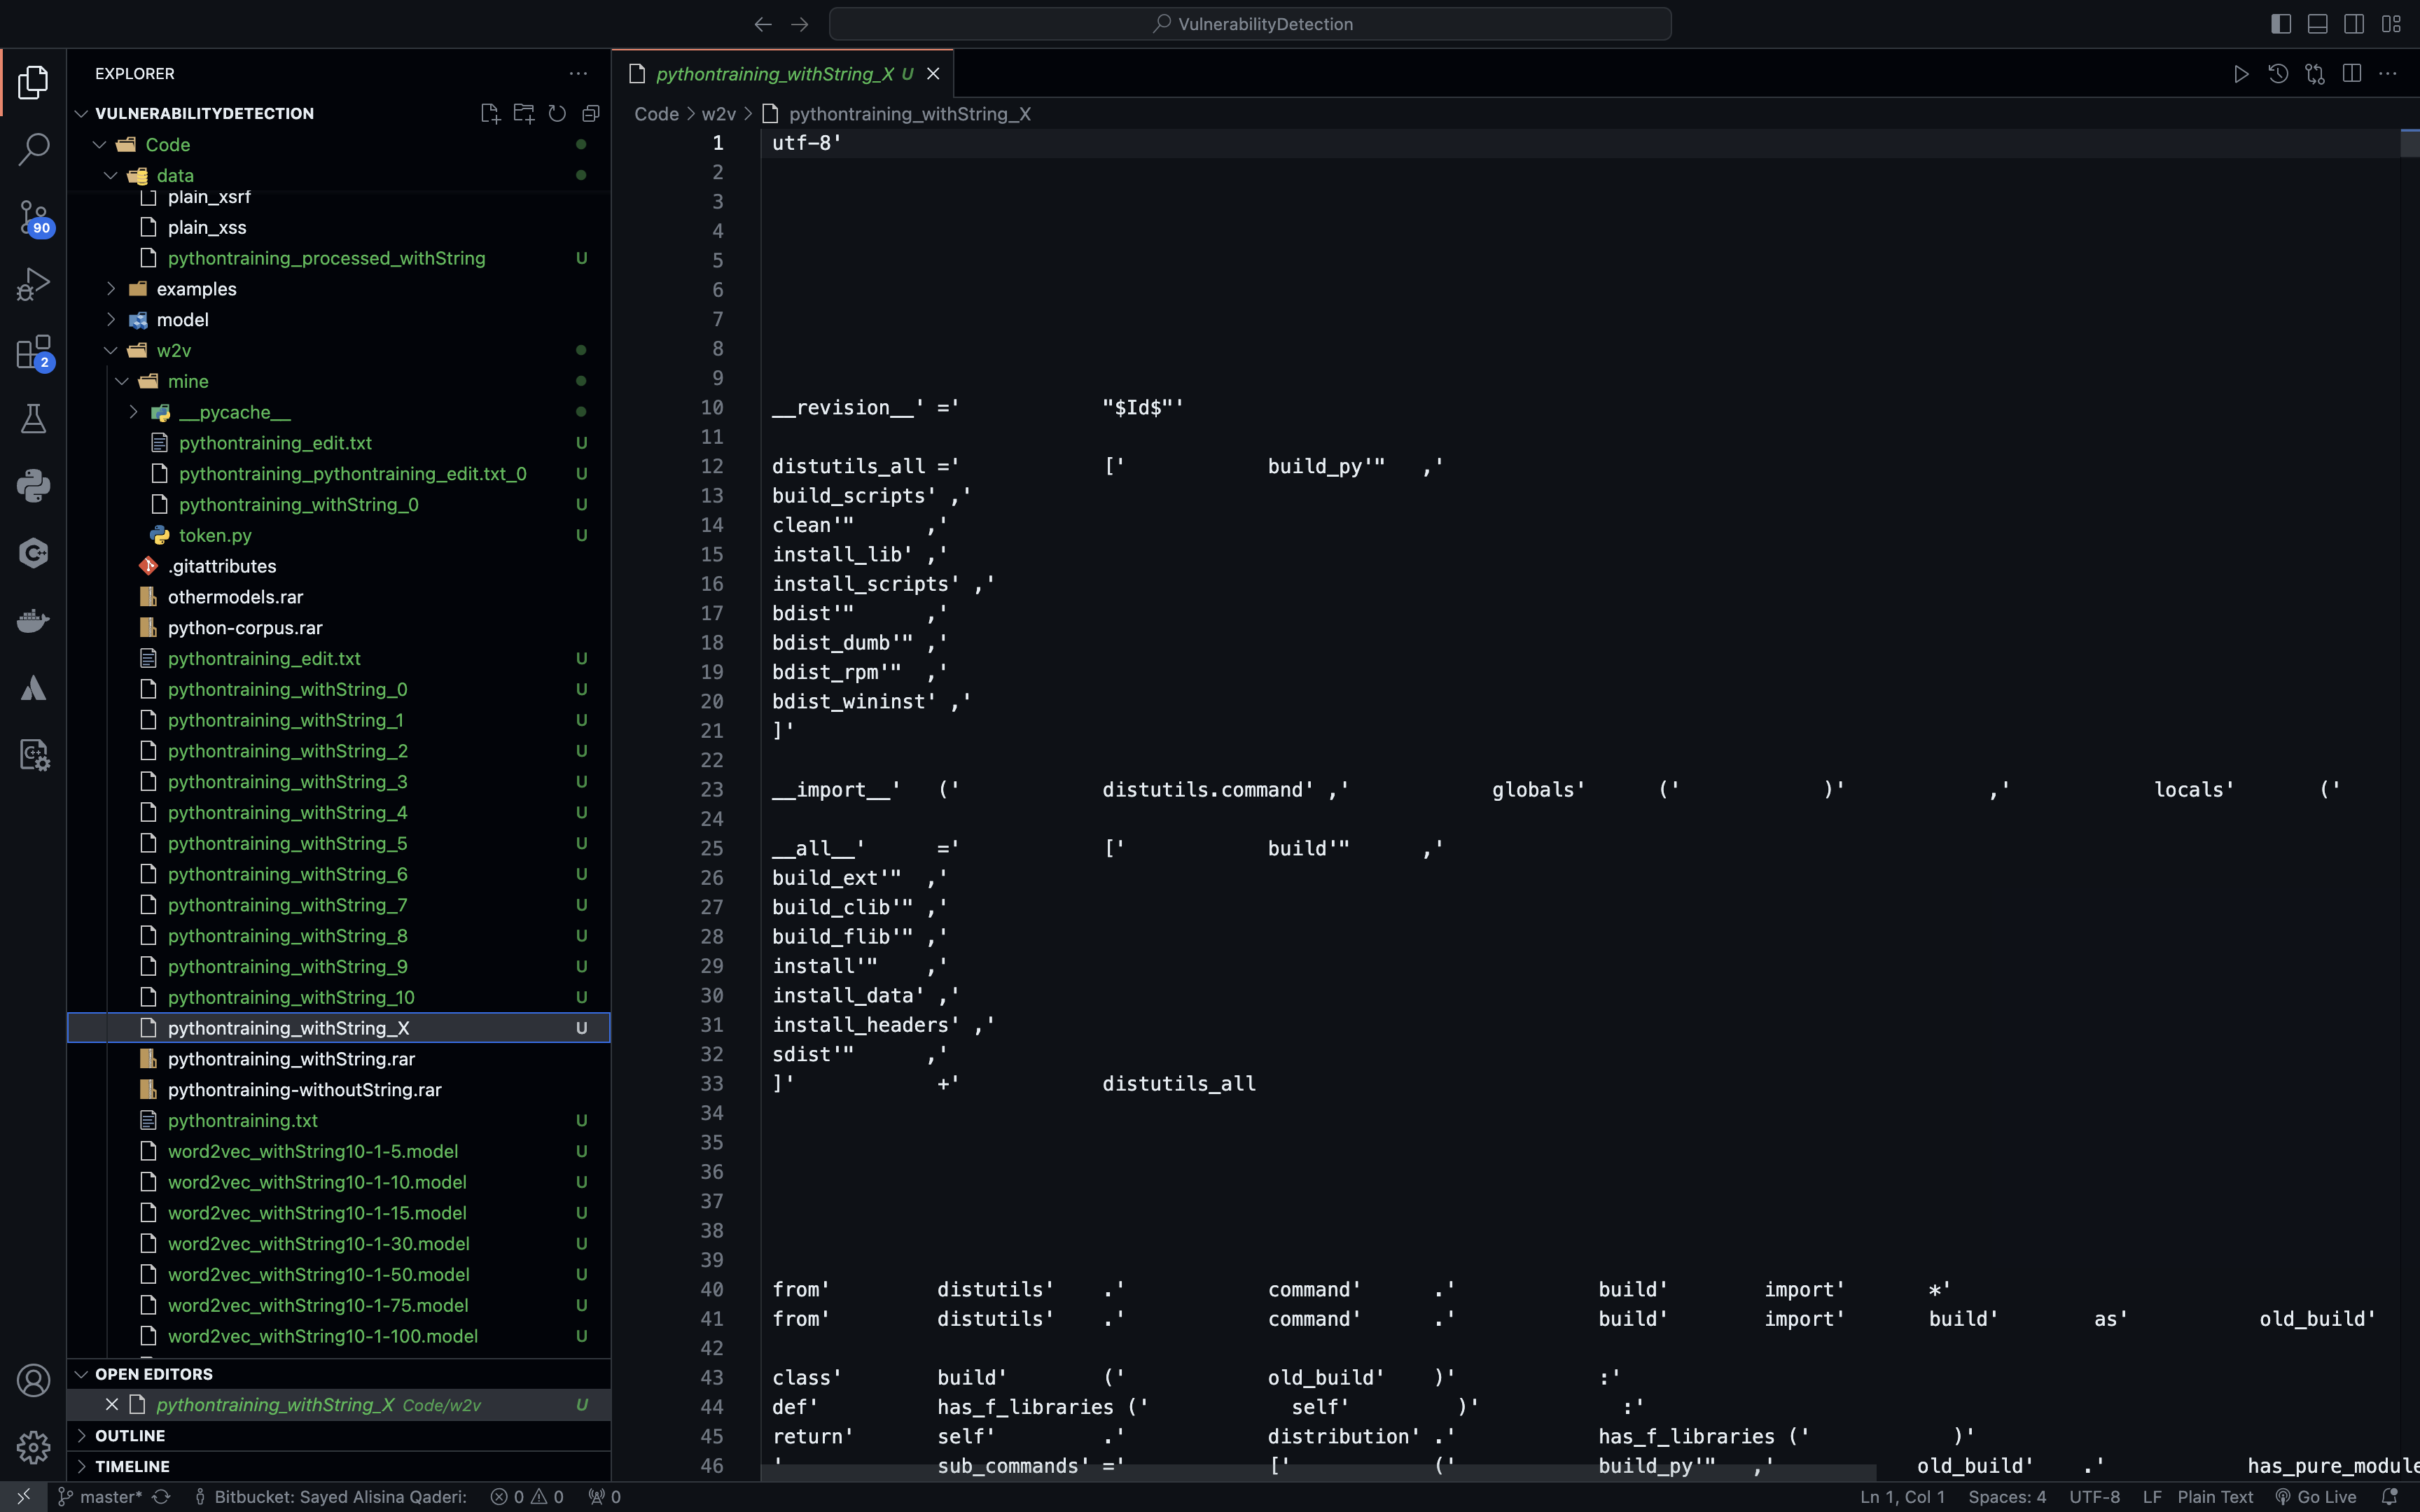
\includegraphics[width=1\linewidth]{pictures/merged_files.png}
    \caption{Merged file}
    \label{fig: Figure7}
\end{figure}

\subsection{\textbf{Training Word2Vec Model}}
In this step, we will generate our model based on tokenized data. While working on this step, we faced some coding issues, which we will explain.
\begin{enumerate}
\item This step required the NLTK library. NLTK has built-in support for dozens of corpora and trained models. To install this library, we should use the following command in the terminal:
    \begin{enumerate}
        \item Mac/Unix: \textit{pip install --user -U nltk}
        \item Windows (32 bit): \textit{pip install nltk} 
        \item As Third Party Software check the following link: \newline \href{https://github.com/nltk/nltk/wiki/Installing-Third-Party-Software}{https://github.com/nltk/nltk/wiki/Installing-Third-Party-Software}
    \end{enumerate}
    After installing the NLTK package, please install the necessary datasets/models for specific functions to work.
    If you’re unsure of which datasets/models you’ll need, you can install the “popular” subset of NLTK data on the command line type \verb |python -m nltk.downloader popular|, or in the Python interpreter \verb|import nltk; nltk.download('popular')| \cite{nltk}
    
    Also, in our case, we have installed only the "punket" model, which was a missing part from NLTK. We solved the problem with "nltk.download('punkt')."
\item Another issue was the deprecation of the Word2Vec library initialization and the ".vocab" variable. It is shown in Figure \ref{fig: Figure8} which changed to ".index\_to\_key"
\item Based on the task description, we should have one model with \textit{paramcount = 10, iterations = 200, and vector size(s) = 300} parameters. 
\newline The iterations=200 was missing, so we manually added it to the array. It is shown in Figure \ref{fig: Figure9}.
\end{enumerate}
\begin{figure}
    \centering
    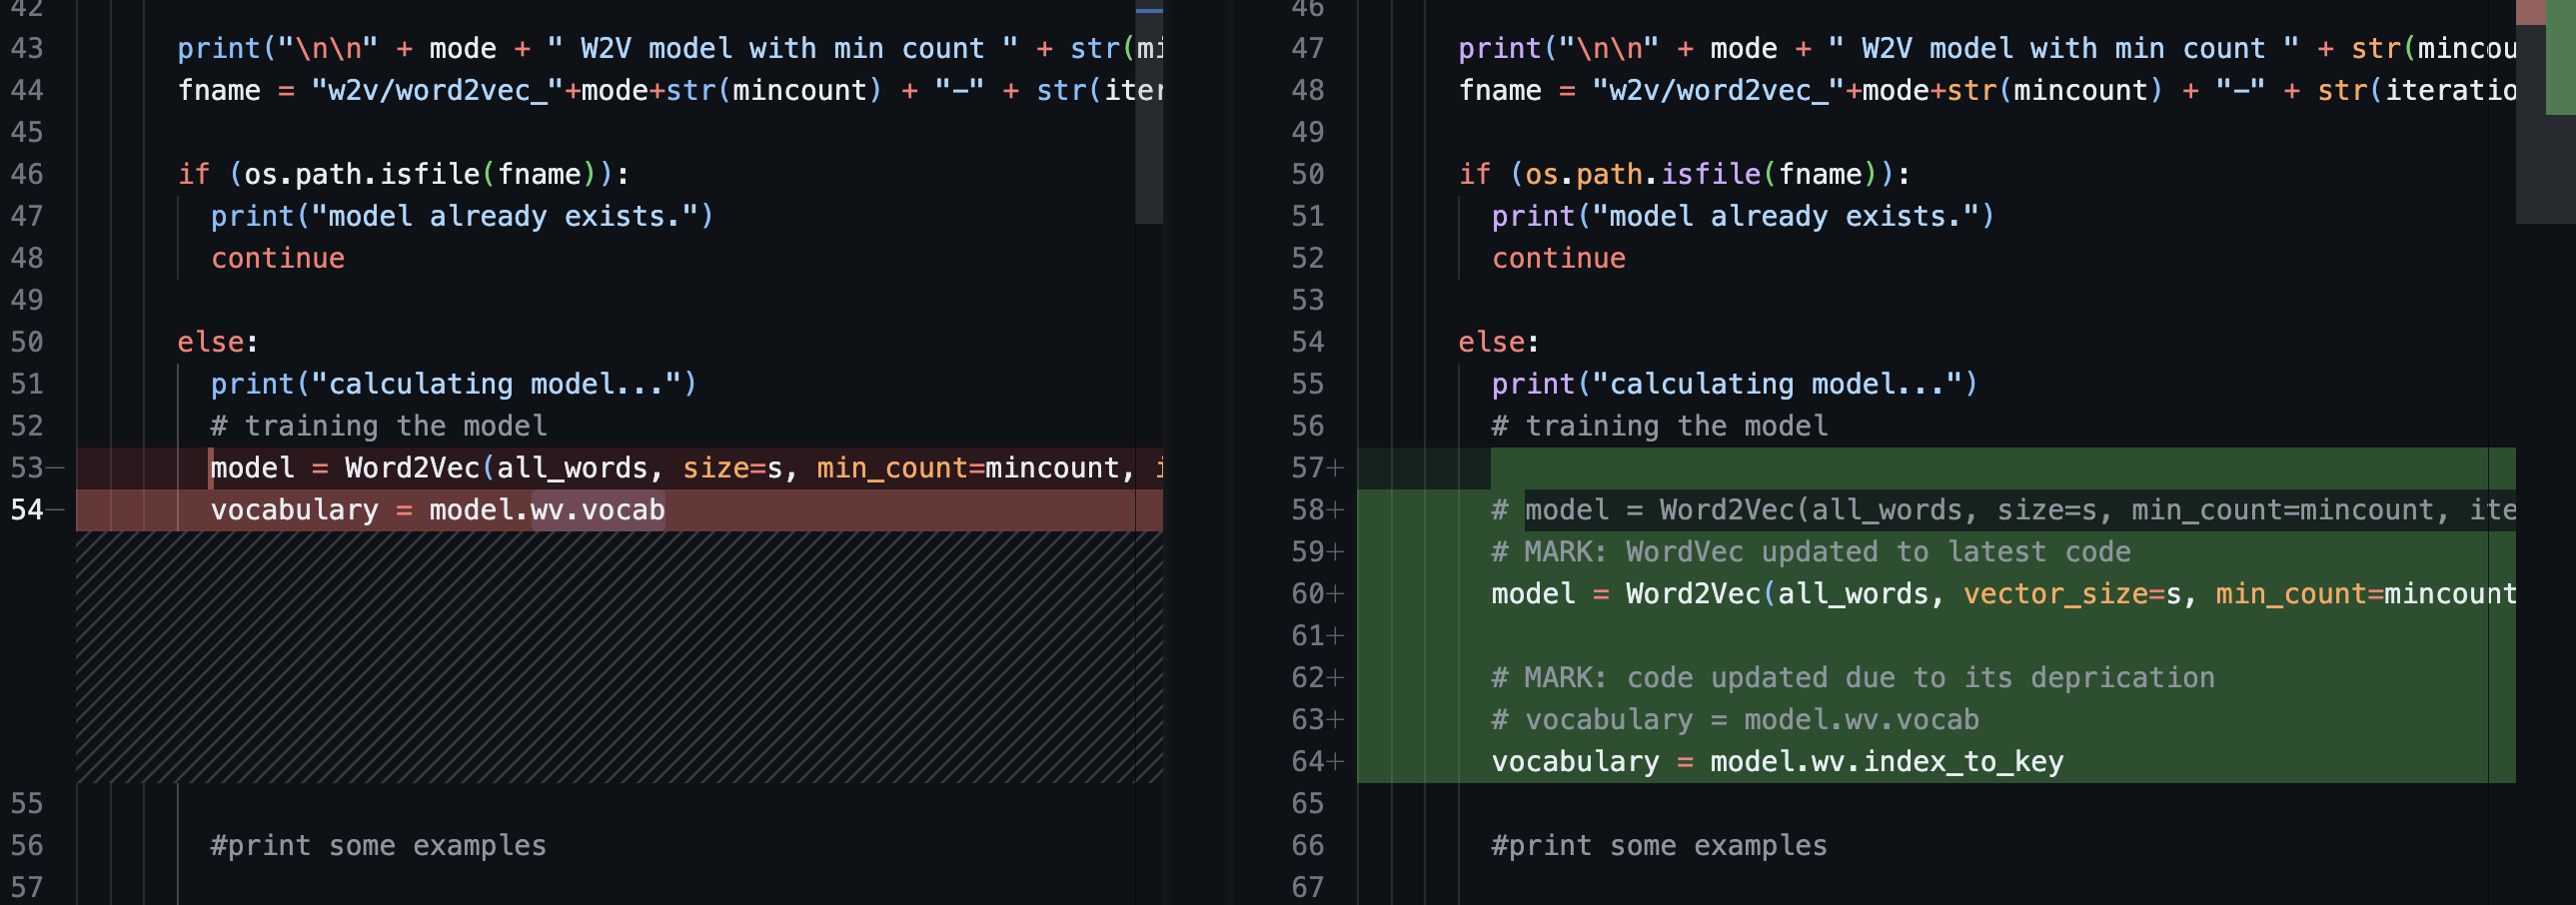
\includegraphics[width=1\linewidth]{pictures/word2vec_deprication.png}
    \caption{Word2Vec Deprecated Code \& Update Code}
    \label{fig: Figure8}
\end{figure}

\begin{figure}
    \centering
    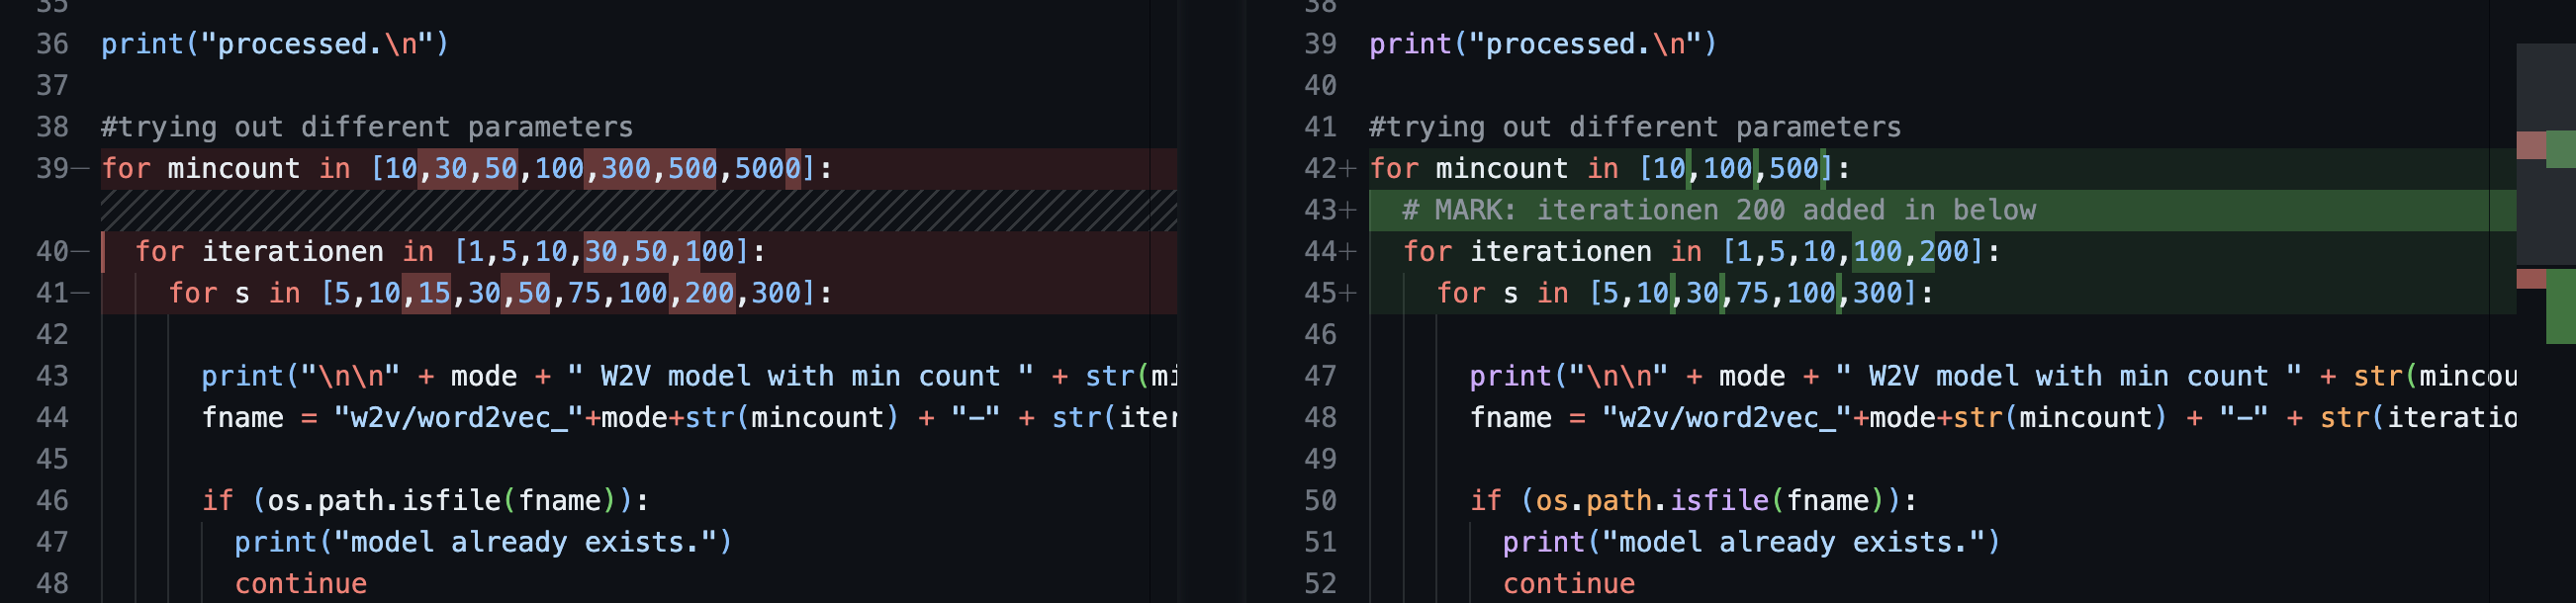
\includegraphics[width=1\linewidth]{pictures/missing_value.png}
    \caption{Missing Iteration Value}
    \label{fig: Figure9}
\end{figure}

After addressing the mentioned issues and implementing the necessary changes, our model training process proceeded successfully with the following parameters (refer to Figure 9):
\begin{itemize}
    \item mincount: [10, 100, 500]
    \item iterations: [1, 5, 10, 100, 200]
    \item vector size (s): [5, 10, 30, 75, 100, 300]
\end{itemize}
These parameters were chosen to optimize our model's performance while considering factors like word frequency thresholds (mincount), training iterations (iterations), and vector size (s).

Additionally, we implemented optimizations to enhance efficiency in both time and space utilization.

As a result of our training, we generated a total of 90 .model files, each representing a trained model. You can observe the model training process in Figure \ref{fig: Figure10}.
\begin{figure}
    \centering
    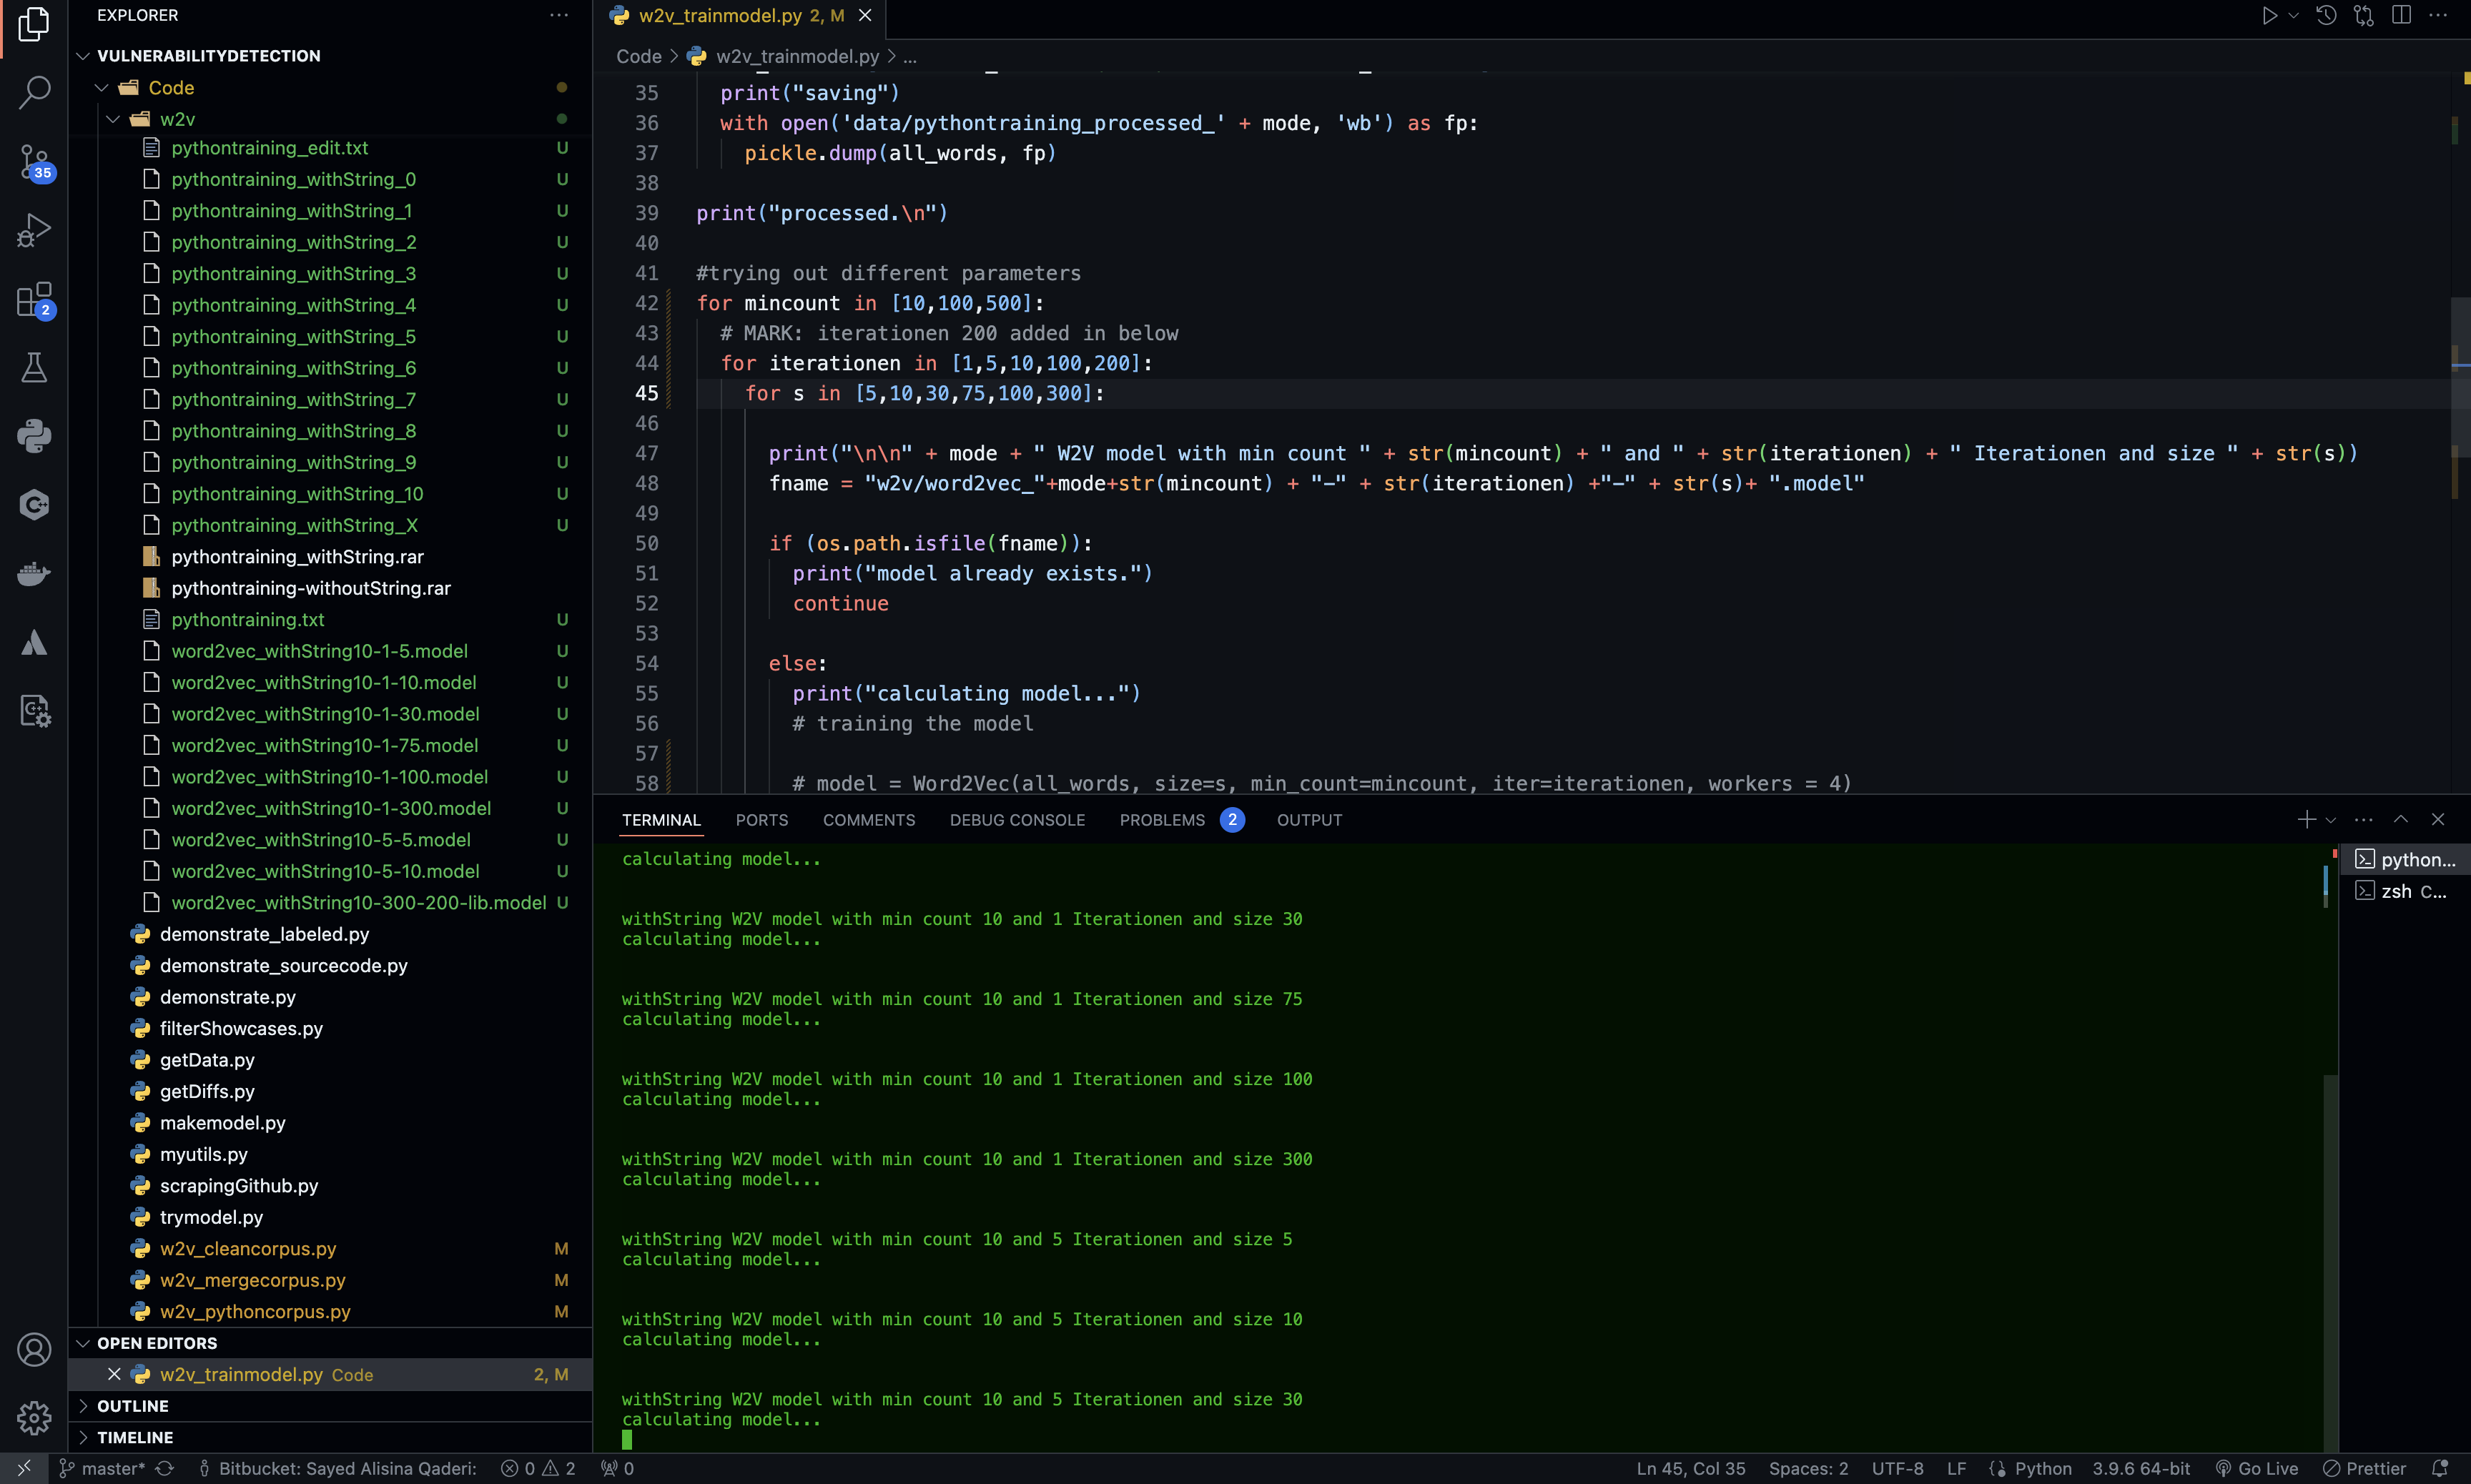
\includegraphics[width=1\linewidth]{pictures/model_training.png}
    \caption{Model Training}
    \label{fig: Figure10}
\end{figure}
\newline
The models will be shared along with this report as archived.
